\documentclass[11pt]{article}
\usepackage[margin=1in]{geometry}
\usepackage{amsmath, amssymb, amsthm, mathtools}
\usepackage{enumitem}
\usepackage{booktabs}
\usepackage[hypertexnames=false]{hyperref}
\usepackage{bm}
\usepackage[section]{placeins}
\usepackage{float}

\hypersetup{
    colorlinks=true,
    linkcolor=blue,
    citecolor=blue,
    urlcolor=blue
}

% ----------------------------- 
% Theorem environments 
% -----------------------------
\theoremstyle{plain}
\newtheorem{theorem}{Theorem}[section]
\newtheorem{proposition}[theorem]{Proposition}
\newtheorem{lemma}[theorem]{Lemma}
\newtheorem{corollary}[theorem]{Corollary}

\theoremstyle{definition}
\newtheorem{definition}[theorem]{Definition}
\newtheorem{construction}[theorem]{Construction}

\theoremstyle{remark}
\newtheorem{remark}[theorem]{Remark}

% -----------------------------
% Proof heading formatting
% -----------------------------
\makeatletter
\renewenvironment{proof}[1][\proofname]{\par\pushQED{\qed}\normalfont
\topsep6\p@\@plus6\p@\relax
\trivlist\item[\hskip\labelsep\bfseries #1\@addpunct{.}]\mbox{}\\\ignorespaces}{\popQED\endtrivlist\@endpefalse}
\makeatother

% ----------------------------- 
% Macros 
% -----------------------------
\newcommand{\R}{\mathbb{R}}
\newcommand{\Rnn}{\mathbb{R}_{\geq 0}}  % nonnegative reals
\newcommand{\Rpp}{\mathbb{R}_{> 0}}     % positive reals
\newcommand{\D}{\mathbb{D}}
\newcommand{\norm}[1]{\left\lVert #1 \right\rVert}
\newcommand{\fnorm}[1]{\left\lVert #1 \right\rVert_F}
\newcommand{\abs}[1]{\left\lvert #1 \right\rvert}
\newcommand{\inner}[2]{\langle #1, #2 \rangle}
\newcommand{\Tr}{\mathrm{Tr}}
\newcommand{\Det}{\mathrm{det}}
\newcommand{\Id}{\mathrm{Id}}
\newcommand{\sgn}{\mathrm{sgn}}
\DeclareMathOperator{\arctanh}{arctanh}
\DeclareMathOperator{\arcosh}{arcosh}

\setcounter{secnumdepth}{3}
\setcounter{tocdepth}{3}

\title{\textbf{A Computable Map from LMS Cone Space \\to the Rebit Bloch Disk}}
\author{%
Guy Singer$^{1}$ \qquad Nir Sochen$^{2}$\\[0.5em]
\small $^{1}$Department of Neurobiology, Tel Aviv University\\
\small $^{2}$Department of Applied Mathematics, Tel Aviv University%
}
\date{\today}

\begin{document}
\maketitle

\begin{abstract}

Recent work models the chromatic state space of human color perception as a Bloch disk, the state space of a real quantum bit, equipped with Klein/Hilbert hyperbolic geometry. These theories are intrinsic, characterizing the abstract geometry without specifying a computable map from physiological cone responses to the disk coordinates. We construct an explicit, parameterized chromaticity map from LMS cone space to the open unit disk via opponent-coordinate formation, luminance normalization, and radial compression, and prove that it is a smooth, disk-bounded, non-surjective map. We establish a luminance-conditioned right inverse with explicit feasibility conditions, equip the disk with the Hilbert metric, and define chromatic attributes through the induced density-matrix embedding. A reference implementation demonstrates numerical stability across standard display gamuts, real-image processing behavior, controlled chromatic-adaptation experiments, parameter/conversion ablations, and a MacAdam-ellipse calibration pilot. The empirical results support the construction as a reproducible computational bridge while leaving psychophysical validation as a separate calibration problem.
\end{abstract}

\newpage
\tableofcontents
\newpage

% =====================================================================
% NEW ABSTRACT
% =====================================================================
% Replace the existing \begin{abstract}...\end{abstract} block with:


% =====================================================================
% NEW INTRODUCTION AND MATHEMATICAL PRELIMINARIES
% =====================================================================
% This replaces any existing \section{Introduction} and adds a
% \section{Mathematical Preliminaries} before the existing Part I.

\section{Introduction}
\label{sec:introduction}

\subsection{Historical and mathematical context}
\label{ssec:historical}

The mathematical study of human color perception has attracted contributions from an extraordinary lineage of scientists, from Newton~\cite{Newton1704}, Grassmann~\cite{Grassmann1853}, and von~Helmholtz~\cite{Helmholtz1924} through Schr\"odinger~\cite{Schrodinger1920}, Riemann~\cite{Riemann1854}, and, more recently, Resnikoff~\cite{Resnikoff1974}.
The classical axiomatization due to Grassmann, von~Helmholtz, and Schr\"odinger establishes, under standard colorimetric observing conditions, that the space~$\mathcal{P}$ of perceived colors is a regular convex cone embedded in a real vector space of dimension at most~$3$.
This structure encodes trichromacy (the linear independence of three primaries), the impossibility of annihilating a nonzero color sensation by superposition (regularity), and the closure of color mixtures under convex combination (convexity).
While powerful, the cone axioms alone impose relatively weak geometric constraints and do not, by themselves, determine a metric capable of quantifying perceptual dissimilarity.

A decisive enrichment was introduced by Resnikoff~\cite{Resnikoff1974}, who postulated that $\mathcal{P}$ is homogeneous under the action of a group $\mathrm{GL}^+(\mathcal{P})$ of linear background-illumination changes.
Provenzi~\cite{Provenzi2020} provided a thorough modern re-examination of this program, supplying a simplified proof of the classification theorem and highlighting two critical open issues: the linearity of background transformations has never been experimentally verified, and the Riemannian metrics singled out by Resnikoff's invariance axiom are incompatible with the crispening effect, whereby color-discrimination thresholds depend systematically on the surround.

\subsection{The Jordan-algebraic and quantum-information-theoretic reformulation}
\label{ssec:jordan}

Berthier~\cite{Berthier2020} proposed an alternative foundation that replaces the external homogeneity postulate with a single structural axiom: the Grassmann--von~Helmholtz cone is the positive cone of a formally real Jordan algebra of real dimension~$3$.
The Jordan--von~Neumann--Wigner classification~\cite{Jordan1934} then restricts $\mathcal{P}$ to be the positive cone of either $\mathbb{R} \oplus \mathbb{R} \oplus \mathbb{R}$ (the flat case, recovering~$\mathcal{P}_1$) or $H(2,\mathbb{R})$, the algebra of $2 \times 2$ real symmetric matrices equipped with the Jordan product $A \circ B = \frac{1}{2}(AB + BA)$.
The latter is isomorphic to the spin factor $\mathbb{R} \oplus \mathbb{R}^2$ endowed with the Minkowski metric, and its state space, the set of positive semidefinite elements with unit trace, is a two-dimensional Bloch disk~$\mathbb{D}$, the state space of a rebit (real quantum bit).

This reformulation brings the apparatus of quantum information theory to bear on color perception.
The chromatic state of a perceived color is identified with a point $v = (v_1, v_2)$ in the open unit disk, and the corresponding density matrix
\[
\rho(v) = \tfrac{1}{2}\bigl(I_2 + v_1 \sigma_1 + v_2 \sigma_2\bigr),
\]
where $\sigma_1, \sigma_2$ are the real Pauli-like generators, encodes opponency in a manner that is axiomatically rather than \emph{ad hoc} motivated.
Pure chromatic states (spectral hues, in the perceptual idealization) lie on the boundary~$\partial\mathbb{D}$; the achromatic state~$\rho_0 = I_2/2$ occupies the center; and the von~Neumann entropy $S(\rho) = -\mathrm{Tr}(\rho \log \rho)$ furnishes an information-theoretic definition of saturation.
Crucially, the natural geometry on~$\mathbb{D}$ is that of the Klein (Beltrami--Klein) disk: the Hilbert metric, whose geodesics are Euclidean chords and whose distance is given by the logarithm of a cross-ratio~\cite{Berthier2020, Beardon1999}.

Subsequent work by Berthier, Provenzi, and collaborators has extended this framework substantially: reconciling trichromacy with opponency via hyperbolicity~\cite{BerthierProvenzi2021hyp}; establishing uncertainty relations for chromatic opposition~\cite{BerthierProvenzi2021unc}; demonstrating that perceived-color relativistic phenomena (originally argued by Yilmaz~\cite{Yilmaz1962}) arise naturally from Lorentz boosts on the rebit state space~\cite{Berthier2021rel}; developing a systematic quantum-measurement theory for color attributes~\cite{BerthierProvenzi2022proc}; and providing a quantum-information-based refoundation of classical colorimetric concepts such as brightness, lightness, chroma, and hue~\cite{BerthierPrencipeProvenzi2022}.

\subsection{The gap: from intrinsic geometry to computable coordinates}
\label{ssec:gap}

Despite the mathematical depth of the intrinsic program, a concrete and computationally implementable mapping from physiological or device color representations to the rebit state coordinates has not been specified.
The Bloch-disk description is explicitly presented ``without reference to physical colors or to an observer''~\cite{Berthier2020}, and the question of how to embed, say, LMS cone responses or CIE~XYZ tristimulus values into $(v_1, v_2) \in \mathbb{D}$ is left open.
This is not merely a practical inconvenience.
Without such a bridge the geometric predictions of the theory (hyperbolic distances, geodesic interpolation, entropy-based saturation) cannot be evaluated on real color data or images, the connection between the abstract opponent generators $\sigma_1, \sigma_2$ and the physiologically grounded opponent channels ($L{-}M$, $S{-}(L{+}M)$) remains purely analogical rather than quantitative, and the calibration against psychophysical data (e.g., MacAdam ellipses~\cite{MacAdam1942}, color-difference datasets) and the estimation of observer-specific convex domains with Finsler geometry, as envisaged by Berthier~\cite{Berthier2020}, cannot be initiated.

\subsection{Contributions}
\label{ssec:contributions}

This work constructs and analyzes an explicit, parameterized chromaticity map
\[
\Phi_\theta = T_\kappa \circ \Pi \circ \mathcal{O} \colon \mathcal{L} = \mathbb{R}_{>0}^3 \longrightarrow \mathbb{D}
\]
that provides a computable bridge from LMS cone space to the chromatic Bloch disk.
The map is composed of three stages: an invertible linear opponent transform~$\mathcal{O}$, a luminance-normalizing projection~$\Pi$, and a smooth radial compression $T_\kappa$ via $\tanh$, and is parameterized by a vector $\theta = (w_L, w_M, \gamma_{LM}, \beta, \varepsilon, \kappa)$ whose components have transparent physiological and geometric interpretations. The specific contributions are as follows.

\paragraph{(1) Construction and analysis.}
We prove that $\Phi_\theta$ is smooth, disk-bounded, and maps the achromatic locus to the maximally mixed state.
We derive the exact attainable region in pre-compression chromaticity coordinates, $u(\mathcal{L}) \subset \R^2$ with $u = \Pi \circ \mathcal{O}$, showing that $u(\mathcal{L})$ is an open half-strip with an affine boundary determined by LMS positivity, and prove that this region is independent of the regularization parameter~$\varepsilon$.
Consequently, $\Phi_\theta(\mathcal{L}) = T_\kappa(u(\mathcal{L})) \subsetneq \mathbb{D}$.
We establish that $\Phi_\theta$ is non-surjective (with explicit excluded intervals on each opponent axis) and construct a luminance-conditioned right inverse with explicit positivity conditions for feasible reconstruction.

\paragraph{(2) Hilbert/Klein geometry and chromatic attributes.}
We implement the Hilbert metric on~$\mathbb{D}$ via both the cross-ratio definition and the closed-form Klein formula, verify their numerical agreement, and derive the metric tensor, geodesic structure, and gyrovector (Klein) addition law.
Chromatic attributes (hue as the angular coordinate of the Bloch vector, saturation as one minus the von~Neumann entropy) are defined in terms of the density-matrix embedding.

\paragraph{(3) Reference implementation and numerical characterization.}
A Python package realizes the full pipeline, including forward map, reconstruction, Hilbert distance, Klein gyroaddition, Jacobian and pullback metric computation, and quantum distances (trace, Bures, fidelity).
We characterize its numerical precision across compression regimes and quantify practical operating ranges for standard display gamuts (sRGB, Display~P3, Rec.~2020).

\paragraph{(4) Explicit non-claims and calibration interface.}
We do not claim that $\Phi_\theta$ is the unique or perceptually correct embedding; we do not resolve the open questions about linearity of background transformations or crispening-compatible metrics; and we do not assert empirical validity across observers.
The parameterization by~$\theta$ is designed to serve as the interface for future psychophysical calibration, fitting $\theta$ so that Hilbert-disk distances predict discrimination thresholds, estimating observer-specific convex domains~$\Omega \subset \mathbb{D}$ whose Hilbert/Finsler geometry matches MacAdam ellipses, and modeling context effects via structured state maps, which we outline as directions for subsequent work.

\subsection{Relation to other approaches}
\label{ssec:related}

The present construction should be distinguished from several related but distinct lines of work.
Classical CIE-derived color-difference formulas (CIELAB, CIEDE2000) are empirically fitted metrics on \emph{ad hoc} coordinate systems that lack an axiomatic geometric foundation~\cite{Wyszecki1982}.
Classical opponent or approximately uniform color spaces such as IPT~\cite{EbnerFairchild1998}, ICtCp~\cite{BT2100}, and OSA-UCS~\cite{Wyszecki1982} provide practically useful opponent coordinates for imaging applications, including LMS-based pipelines, but they are not formulated in terms of the Jordan-algebraic or rebit-state geometry considered here.
Riemannian models of color space~\cite{Resnikoff1974, Provenzi2020} operate intrinsically on the perceived-color cone and derive metrics from invariance principles, but do not incorporate the Jordan-algebraic or quantum structure.
The quantum-information program of Berthier--Provenzi~\cite{Berthier2020, BerthierProvenzi2021hyp, BerthierPrencipeProvenzi2022} provides the target geometry that our map is designed to reach, but operates intrinsically without an explicit coordinate embedding from cone responses.
Our contribution is thus a bridge: it takes as given the standard colorimetric pipeline (sRGB~$\to$~XYZ~$\to$~LMS) on the input side and the rebit Bloch disk on the output side, and provides a mathematically controlled, parameterized map connecting them. The novelty is therefore not the bare introduction of opponent coordinates, but the specific geometric target and the disk-bounded compression that carries LMS-derived chromaticity into that target space.

\subsection{Organization}
\label{ssec:organization}

After the introduction, Section~\ref{sec:framework} develops the mathematical framework. Section~\ref{sec:construction-properties} presents the construction and properties of the chromaticity map. Section~\ref{sec:disk-geometry} studies the geometry and chromatic attributes of the Bloch disk. Sections~\ref{sec:results}--\ref{sec:reproducibility} then describe the numerical implementation and experiments, discussion, and reproducibility details.
%=============================================================================
\section{Mathematical Framework}
\label{sec:framework}
%=============================================================================

\paragraph{Notation.} Throughout the mathematical sections, we use:
\begin{itemize}
    \item $\Rpp := (0, \infty)$ for strictly positive reals and $\Rnn := [0, \infty)$ for nonnegative reals.
    \item $\norm{v} := \sqrt{v_1^2 + v_2^2}$ for the Euclidean norm on $\R^2$. $\fnorm{\cdot}$ denotes the Frobenius norm for matrices.
    \item $\inner{u}{v} := u_1 v_1 + u_2 v_2$ for the Euclidean inner product on $\R^2$.
    \item $\partial \D := \{v \in \R^2 : \norm{v} = 1\}$ for the boundary of the disk $\D$.
    \item $X \succeq 0$ means the matrix $X$ is positive semidefinite (all eigenvalues $\geq 0$).
\end{itemize}

%=============================================================================
\subsection{The Target Space: Rebit State Space}
\label{sec:target}
%=============================================================================

We begin by establishing the mathematical structure of the target space. A rebit (``real qubit'') is a two-level quantum system described by real (rather than complex) amplitudes. Its state space is the set of $2 \times 2$ real symmetric positive semidefinite matrices with unit trace, which we parameterize by the Bloch disk $\D$.

We denote by $H(2,\R)$ the set of $2 \times 2$ real symmetric matrices,
\begin{equation}
H(2,\R) = \left\{ X \in \R^{2\times 2} : X^T = X \right\},
\end{equation}
viewed as a $3$-dimensional real vector space equipped with the Jordan product $A \circ B = \frac{1}{2}(AB + BA)$. Every element $X \in H(2,\R)$ admits a unique decomposition
\begin{equation}
X = \alpha \Id_2 + m_1 \sigma_1 + m_2 \sigma_2,
\end{equation}
where $\alpha \in \R$, $(m_1, m_2) \in \R^2$, and
\begin{equation}
\Id_2 = \begin{pmatrix} 1 & 0 \\ 0 & 1 \end{pmatrix}, \quad
\sigma_1 = \begin{pmatrix} 1 & 0 \\ 0 & -1 \end{pmatrix}, \quad
\sigma_2 = \begin{pmatrix} 0 & 1 \\ 1 & 0 \end{pmatrix}.
\end{equation}
Indeed, writing $X = \begin{pmatrix} a & b \\ b & c \end{pmatrix}$ gives $\alpha = \frac{a+c}{2}$, $m_1 = \frac{a-c}{2}$, and $m_2 = b$, while uniqueness follows from the linear independence of $\{\Id_2, \sigma_1, \sigma_2\}$. It is therefore natural to introduce the linear map $\chi: H(2,\R) \to \R \oplus \R^2$ by
\begin{equation}
\chi\left( \begin{pmatrix} \alpha + m_1 & m_2 \\ m_2 & \alpha - m_1 \end{pmatrix} \right) = (\alpha, m_1, m_2),
\end{equation}
which is an isomorphism preserving the quadratic form in the sense that $\Det(X) = \alpha^2 - \norm{m}^2$.

The positive cone $H_+(2,\R) \subset H(2,\R)$ is
\begin{equation}
H_+(2,\R) = \{ X \in H(2,\R) : X \succeq 0 \} = \{ X : \Tr(X) \geq 0, \Det(X) \geq 0 \}.
\end{equation}
For symmetric $2 \times 2$ matrices, the characterization by trace and determinant is equivalent to positive semidefiniteness because the eigenvalues are real, and they are both nonnegative precisely when their sum and product are nonnegative. The chromatic state space is then modeled by the open unit disk
\begin{equation}
\D = \{ v \in \R^2 : \norm{v} < 1 \},
\end{equation}
with closed disk $\bar{\D} = \{ v \in \R^2 : \norm{v} \leq 1 \}$. For $v = (v_1, v_2) \in \bar{\D}$ we associate the density matrix
\begin{equation}
\boxed{
\rho(v) = \frac{1}{2}\left( \Id_2 + v_1 \sigma_1 + v_2 \sigma_2 \right) = \frac{1}{2} \begin{pmatrix} 1 + v_1 & v_2 \\ v_2 & 1 - v_1 \end{pmatrix}.
}
\end{equation}
Under $\chi$, one has $\chi(\rho(v)) = (\frac{1}{2}, \frac{v_1}{2}, \frac{v_2}{2})$, so the Bloch vector $v$ is twice the spatial Minkowski coordinate.

\begin{proposition}
\label{prop:density-props}
For $v \in \bar{\D}$, the matrix $\rho(v)$ satisfies:
\begin{enumerate}[label=(\roman*)]
    \item $\rho(v) \succeq 0$ (positive semidefinite, i.e., all eigenvalues $\geq 0$)
    \item $\Tr(\rho(v)) = 1$ (unit trace)
    \item $\rho(v)^2 = \rho(v)$ if and only if $\norm{v} = 1$ (pure state condition)
    \item The eigenvalues are $\lambda_{\pm} = \frac{1}{2}(1 \pm \norm{v})$
\end{enumerate}
A pure state ($\norm{v} = 1$) represents maximal chromatic information; a mixed state
($\norm{v} < 1$) represents partial chromatic information, with the maximally mixed state
at $v = (0,0)$. Conversely, every $2 \times 2$ real symmetric positive semidefinite matrix with trace $1$
has a unique $v \in \bar{\D}$ such that $\rho = \rho(v)$.
\end{proposition}

\begin{proof}
\textbf{(i)--(ii)} Direct computation gives
\begin{align*}
\Tr(\rho(v)) &= 1, \\
\Det(\rho(v)) &= \frac{1}{4}\bigl(1 - \norm{v}^2\bigr) \geq 0, \qquad (\norm{v} \leq 1).
\end{align*}

\noindent\textbf{(iii)} Using $\sigma_i^2 = \Id_2$ for $i \in \{1,2\}$ and $\sigma_1\sigma_2 + \sigma_2\sigma_1 = 0$, we compute
\begin{align*}
\rho(v)^2
&= \frac{1}{4}\bigl(\Id_2 + v_1\sigma_1 + v_2\sigma_2\bigr)^2 \\
&= \frac{1}{4}\Bigl( (1 + \norm{v}^2)\Id_2 + 2v_1\sigma_1 + 2v_2\sigma_2 \Bigr).
\end{align*}
\noindent This equals $\rho(v)$ if and only if $1 + \norm{v}^2 = 2$, i.e., $\norm{v} = 1$.

\noindent\textbf{(iv)} The characteristic polynomial is
\[
\lambda^2 - \lambda + \frac{1}{4}\bigl(1 - \norm{v}^2\bigr) = 0.
\]

\noindent\textbf{Converse.} Let
\[
\rho = \begin{psmallmatrix} a & b \\ b & c \end{psmallmatrix},
\qquad \rho \succeq 0, \qquad a + c = 1.
\]
\noindent Define
\begin{align*}
v_1 &:= a - c = 2a - 1, \\
v_2 &:= 2b.
\end{align*}
\noindent Then
\begin{align*}
\rho(v)
&= \frac{1}{2}\begin{pmatrix} 1 + v_1 & v_2 \\ v_2 & 1 - v_1 \end{pmatrix} \\
&= \frac{1}{2}\begin{pmatrix} 2a & 2b \\ 2b & 2c \end{pmatrix}
 = \begin{pmatrix} a & b \\ b & c \end{pmatrix}
 = \rho.
\end{align*}
\noindent Moreover,
\begin{align*}
\Det(\rho)
&= ac - b^2 \\
&= \frac{(1+v_1)(1-v_1)}{4} - \frac{v_2^2}{4} \\
&= \frac{1 - \norm{v}^2}{4}.
\end{align*}
\noindent Thus $\rho \succeq 0$ implies $\Det(\rho) \geq 0$ and hence $\norm{v} \leq 1$.
\noindent Uniqueness follows from $v_1 = a - c$ and $v_2 = 2b$.
\end{proof}

The achromatic state corresponds to $v = (0,0)$, hence
\begin{equation}
\rho_0 := \rho(0,0) = \frac{1}{2}\Id_2.
\end{equation}
It is the maximally mixed state, with eigenvalues $\lambda_+ = \lambda_- = \frac{1}{2}$.

%=============================================================================
\subsection{The Source Space: LMS Cone Responses}
\label{sec:source}
%=============================================================================

The LMS cone response space is
\begin{equation}
\mathcal{L} = \Rpp^3 = \{ (L, M, S) \in \R^3 : L > 0, M > 0, S > 0 \}.
\end{equation}
Here $L$, $M$, and $S$ denote the responses of the three retinal cone classes, named for their peak sensitivities to \textbf{L}ong, \textbf{M}edium, and \textbf{S}hort wavelengths. We impose strict positivity in order to exclude degenerate boundary cases. For a spectral power distribution $C(\lambda)$ over the visible range, these responses take the form $L = \int C(\lambda) \bar{l}(\lambda) \, d\lambda$, and similarly for $M$ and $S$, where $\bar{l}, \bar{m}, \bar{s}$ are the cone sensitivity functions.

The transformation from CIE XYZ (or RGB) to LMS is external to the present construction: it depends on a chosen $3 \times 3$ matrix, whose entries vary with the selected cone fundamentals (for example Hunt--Pointer--Estevez, CAT02, or Stockman--Sharpe cone fundamentals~\cite{StockmanSharpe2000}). Throughout the mathematical development we therefore treat LMS coordinates as given data. For image data, standard sRGB values must first be gamma-decoded before any linear color transformation is applied; otherwise the resulting LMS coordinates inherit a systematic nonlinearity. In addition, numerical XYZ-to-LMS transforms can produce small negative values for out-of-gamut inputs, so the implementation applies a mild positive clamp to ensure $(L, M, S) \in \mathcal{L}$.

%=============================================================================
\section{Construction and Properties of the Chromaticity Map}
\label{sec:construction-properties}
%=============================================================================

%=============================================================================
\subsection{Construction of the Chromaticity Map}
\label{sec:construction}
%=============================================================================

We construct the map $\Phi_\theta: \mathcal{L} \to \D$ in four stages. We deliberately refer to $\Phi_\theta$ as a \emph{chromaticity map} rather than an embedding, because it is not injective: luminance information is discarded, so the scaling $(L, M, S) \mapsto t(L, M, S)$ leaves the chromatic component essentially unchanged. An injective formulation would require restricting to a fixed-luminance manifold, such as $Y = w_L L + w_M M = 1$, or equivalently passing to ratio coordinates.

\subsubsection{Stage 1: Opponent Coordinate Formation}

Let $w_L, w_M, \gamma_{LM}, \beta \in \Rpp$ be positive parameters. We define a Hering-type opponent coordinate map~\cite{Hering1878} $\mathcal{O}: \mathcal{L} \to \Rpp \times \R^2$ by
\begin{equation}
\mathcal{O}(L, M, S) = \begin{pmatrix} Y \\ O_1 \\ O_2 \end{pmatrix} = \begin{pmatrix} w_L L + w_M M \\ L - \gamma_{LM} M \\ S - \beta(L + M) \end{pmatrix},
\end{equation}
or, in matrix form,
\begin{equation}
\boxed{
\mathcal{O}(L, M, S) = \underbrace{\begin{pmatrix} w_L & w_M & 0 \\ 1 & -\gamma_{LM} & 0 \\ -\beta & -\beta & 1 \end{pmatrix}}_{=: A_\theta} \begin{pmatrix} L \\ M \\ S \end{pmatrix}.
}
\end{equation}
Since
\begin{equation}
\Det(A_\theta) = -(w_L \gamma_{LM} + w_M) \neq 0,
\end{equation}
the matrix $A_\theta$ is invertible for all admissible parameters. We write
\begin{equation}
\Delta := w_L \gamma_{LM} + w_M > 0.
\end{equation}
Our sign convention takes $O_1 = L - \gamma_{LM} M > 0$ to indicate L-cone dominance. Physiological discussions sometimes describe this pole as ``reddish'' rather than ``greenish,'' but the terminology is purely conventional: replacing $O_1$ by $-O_1$ simply exchanges the red-green poles.

\subsubsection{Stage 2: Luminance Normalization}

Let $\varepsilon \in \Rnn$ be a regularization parameter. We then define the chromaticity projection $\Pi: \Rpp \times \R^2 \to \R^2$ by
\begin{equation}
\boxed{
\Pi(Y, O_1, O_2) = u = (u_1, u_2) := \left( \frac{O_1}{Y + \varepsilon}, \frac{O_2}{Y + \varepsilon} \right).
}
\end{equation}
We write $u^{(\varepsilon)}(x) := \Pi \circ \mathcal{O}(x)$ for the regularized chromaticity coordinates and $u^{(0)}(x) := (O_1/Y, O_2/Y)$ for the idealized scale-invariant coordinates, where $Y: \mathcal{L} \to \Rpp$ is the luminance function $Y(x) := w_L L + w_M M$. The case $\varepsilon = 0$ is useful for describing the exact boundary of the attainable set, whereas numerical work typically uses a small positive value of $\varepsilon$ for stability.

\begin{proposition}
\label{prop:scale-invariance}
For $t > 0$ and $x = (L, M, S) \in \mathcal{L}$, let $Y = Y(x) = w_L L + w_M M$ denote the luminance, and let $O := (O_1, O_2) = (L - \gamma_{LM} M, S - \beta(L+M))$ denote the opponent coordinate vector.
Then
\begin{equation}
u^{(\varepsilon)}(tx)
= \frac{tO}{tY + \varepsilon}
= \frac{tY}{tY + \varepsilon} \cdot u^{(0)}(x)
= \frac{t}{t + \varepsilon/Y} \cdot u^{(0)}(x)
= \frac{t(Y + \varepsilon)}{tY + \varepsilon} \cdot u^{(\varepsilon)}(x).
\end{equation}
The first two expressions interpret the scaling relative to the scale-invariant chromaticity $u^{(0)}(x)$, while the last expression gives the corresponding factor relative to the regularized chromaticity $u^{(\varepsilon)}(x)$. In particular, the last factor equals $1$ at $t = 1$. As $t \to \infty$, $u^{(\varepsilon)}(tx) \to u^{(0)}(x)$.
\end{proposition}

\begin{proof}
\noindent Let $x' = tx$. Then $Y' = tY$ and $O' = tO$, so
\[
 u^{(\varepsilon)}(tx) = \frac{tO}{tY + \varepsilon}.
\]
Using $u^{(0)}(x) = O/Y$ gives
\[
u^{(\varepsilon)}(tx)
= \frac{tO}{tY + \varepsilon}
= \frac{tY}{tY + \varepsilon}\cdot \frac{O}{Y}
= \frac{tY}{tY + \varepsilon}\cdot u^{(0)}(x)
= \frac{t}{t + \varepsilon/Y}\cdot u^{(0)}(x).
\]
Using $u^{(\varepsilon)}(x) = O/(Y + \varepsilon)$ then yields
\[
\frac{u^{(\varepsilon)}(tx)}{u^{(\varepsilon)}(x)}
= \frac{tO/(tY + \varepsilon)}{O/(Y + \varepsilon)}
= \frac{t(Y + \varepsilon)}{tY + \varepsilon},
\]
which is equivalent to the final expression in the statement.
\end{proof}

\paragraph{Attainable chromaticity region.}

The positivity constraints $L, M, S > 0$ impose a precise geometric constraint on attainable chromatic coordinates.

\begin{proposition}
\label{prop:u1-bounds}
For all $(L, M, S) \in \mathcal{L}$,
\begin{equation}
-\frac{\gamma_{LM}}{w_M} < u_1^{(0)} < \frac{1}{w_L}.
\end{equation}
Every value in this open interval is attained.
\end{proposition}

\begin{proof}
\noindent Let $t := L/M > 0$ denote the L-to-M cone ratio. Then
\[
 u_1^{(0)} = \frac{O_1}{Y} = \frac{t - \gamma_{LM}}{w_L t + w_M}.
\]

\noindent Define $f : (0,\infty) \to \R$ by
\[
 f(t) := \frac{t - \gamma_{LM}}{w_L t + w_M}.
\]
A direct computation gives
\[
 f'(t) = \frac{w_L\gamma_{LM} + w_M}{(w_L t + w_M)^2} > 0,
\]
so $f$ is strictly increasing. Moreover,
\[
 \lim_{t \to 0^+} f(t) = -\frac{\gamma_{LM}}{w_M},
 \qquad
 \lim_{t \to \infty} f(t) = \frac{1}{w_L}.
\]
This proves the bounds.
\end{proof}

\begin{lemma}
\label{lem:u1-eps-bounds}
For any $\varepsilon \geq 0$ and all $(L, M, S) \in \mathcal{L}$,
\begin{equation}
-\frac{\gamma_{LM}}{w_M} < u_1^{(\varepsilon)} < \frac{1}{w_L}.
\end{equation}
\end{lemma}

\begin{proof}
\noindent We have
\[
 u_1^{(\varepsilon)} = \frac{Y}{Y+\varepsilon}\, u_1^{(0)},
 \qquad
 \frac{Y}{Y+\varepsilon} \in (0,1].
\]

\noindent If $u_1^{(0)} > 0$, then $u_1^{(\varepsilon)} \leq u_1^{(0)} < 1/w_L$.

\noindent If $u_1^{(0)} < 0$, then $u_1^{(\varepsilon)} \geq u_1^{(0)} > -\gamma_{LM}/w_M$.

\noindent If $u_1^{(0)} = 0$, then $u_1^{(\varepsilon)} = 0$.
\end{proof}

\begin{proposition}
\label{prop:attainable-eps0}
Define the idealized chromaticity $u^{(0)}(x) := (O_1/Y, O_2/Y)$. The image $u^{(0)}(\mathcal{L}) \subset \R^2$ is
\begin{equation}
\boxed{
u^{(0)}(\mathcal{L}) = \left\{(u_1,u_2) \in \R^2 :\; -\frac{\gamma_{LM}}{w_M} < u_1 < \frac{1}{w_L},\; u_2 > g(u_1) \right\}
}
\end{equation}
where the lower boundary is the affine function
\begin{equation}
g(u_1) := -\frac{\beta}{\Delta}\Bigl(\gamma_{LM}+1+(w_M-w_L)u_1\Bigr).
\end{equation}
\end{proposition}

\begin{proof}
\noindent\textbf{(Necessity)} Let $t := L/M > 0$ and $s := S/M > 0$. Then
\[
 u_1 = \frac{t - \gamma_{LM}}{w_L t + w_M},
 \qquad
 u_2 = \frac{s - \beta(t+1)}{w_L t + w_M}.
\]
Since $s > 0$, we have
\[
 u_2 > -\frac{\beta(t+1)}{w_L t + w_M}.
\]
Inverting $f(t) = u_1$ gives
\[
 t = f^{-1}(u_1) = \frac{\gamma_{LM} + w_M u_1}{1 - w_L u_1}
 \qquad \text{for } u_1 \in \left(-\frac{\gamma_{LM}}{w_M}, \frac{1}{w_L}\right),
\]
and in particular $t>0$ on this interval.
Substituting into the lower bound yields
\[
-\frac{\beta(t+1)}{w_L t + w_M}
= -\frac{\beta\bigl(\gamma_{LM} + 1 + (w_M - w_L)u_1\bigr)}{\Delta}
= g(u_1).
\]

\noindent\textbf{(Sufficiency)} Conversely, let $(u_1, u_2)$ satisfy $-\gamma_{LM}/w_M < u_1 < 1/w_L$ and $u_2 > g(u_1)$. Define
\[
 t := \frac{\gamma_{LM} + w_M u_1}{1 - w_L u_1} > 0,
 \qquad
 D_t := w_L t + w_M = \frac{\Delta}{1 - w_L u_1} > 0.
\]
Then set
\[
 s := \beta(t+1) + u_2 D_t.
\]
The condition $u_2 > g(u_1)$ is equivalent to $s > 0$.
Choose any $M > 0$ and set
\[
 L := tM > 0,
 \qquad
 S := sM > 0.
\]
Direct substitution verifies $u^{(0)}(L, M, S) = (u_1, u_2)$.
\end{proof}

The set $u^{(0)}(\mathcal{L})$ is open in $\R^2$ because it is defined by the strict inequalities $-\gamma_{LM}/w_M < u_1 < 1/w_L$ and $u_2 > g(u_1)$. Proposition~\ref{prop:attainable-eps0} treats the idealized case $\varepsilon = 0$, which captures the boundary geometry exactly; the next statement shows that the same image set is obtained for every positive regularization.

\begin{corollary}
\label{cor:attainable-epspos}
For any $\varepsilon > 0$, as sets:
\begin{equation}
u^{(\varepsilon)}(\mathcal{L}) = u^{(0)}(\mathcal{L})
\end{equation}
The regularization $\varepsilon > 0$ does not change the attainable chromaticity region; it only changes the parametrization by luminance.
\end{corollary}

\begin{proof}
We establish equality by two inclusions.

\textbf{($\subseteq$):} For any $x \in \mathcal{L}$, we have
\begin{equation}
u^{(\varepsilon)}(x) = \frac{Y(x)}{Y(x) + \varepsilon} \cdot u^{(0)}(x) =: \lambda(x) \cdot u^{(0)}(x),
\end{equation}
where $\lambda(x) := Y(x)/(Y(x) + \varepsilon) \in (0, 1)$ is the luminance attenuation factor. The region $u^{(0)}(\mathcal{L})$ is star-shaped with respect to the origin, meaning: for every $u \in u^{(0)}(\mathcal{L})$ and every $\mu \in [0,1]$, we have $\mu u \in u^{(0)}(\mathcal{L})$. This holds because $g(0) = -\beta(\gamma_{LM}+1)/\Delta < 0$, so $(0,0) \in u^{(0)}(\mathcal{L})$, and the affine boundary with negative intercept ensures radial inward scalings remain in the region. Thus $u^{(\varepsilon)}(x) \in u^{(0)}(\mathcal{L})$.

\textbf{($\supseteq$):} Let $u \in u^{(0)}(\mathcal{L})$. Since $u^{(0)}(\mathcal{L})$ is open and contains $u$, there exists $\delta > 0$ such that the ball $B(u, \delta) \subset u^{(0)}(\mathcal{L})$. Choose $\alpha > 1$ close enough to $1$ so that $\norm{\alpha u - u} = (\alpha - 1)\norm{u} < \delta$; then $\alpha u \in u^{(0)}(\mathcal{L})$. By Proposition~\ref{prop:attainable-eps0} (sufficiency), there exists $x \in \mathcal{L}$ with $u^{(0)}(x) = \alpha u$. Now choose $t > 0$ so that
\begin{equation}
\frac{tY(x)}{tY(x) + \varepsilon} = \frac{1}{\alpha}, \quad \text{i.e.,} \quad t = \frac{\varepsilon}{Y(x)(\alpha - 1)}.
\end{equation}
Then $u^{(\varepsilon)}(tx) = \frac{1}{\alpha} \cdot (\alpha u) = u$, so $u \in u^{(\varepsilon)}(\mathcal{L})$.
\end{proof}

Geometrically, the attainable region $u^{(0)}(\mathcal{L})$ is an open half-strip: a vertical strip in the $u_1$-direction intersected with the half-plane above the affine boundary $u_2 = g(u_1)$. In particular, it is not a rectangle, because the lower bound for $u_2$ depends affinely on $u_1$.

\subsubsection{Stage 3: Radial Compression to the Disk}

Let $\kappa > 0$ be the saturation-rate parameter. We define the radial compression map $T_\kappa: \R^2 \to \D$ by
\begin{equation}
\boxed{
T_\kappa(u) = \begin{cases}
\displaystyle \tanh(\kappa \norm{u}) \cdot \frac{u}{\norm{u}}, & u \neq (0,0), \\[0.8em]
(0,0), & u = (0,0).
\end{cases}
}
\end{equation}

\begin{proposition}
\label{prop:compression-props}
The map $T_\kappa: \R^2 \to \D$ satisfies:
\begin{enumerate}[label=(\roman*)]
    \item $T_\kappa$ is smooth on $\R^2$ (smoothness at $(0,0)$ follows from $\tanh(\kappa r)/r \to \kappa$ as $r \to 0$)
    \item $\norm{T_\kappa(u)} = \tanh(\kappa\norm{u}) < 1$ for all $u \in \R^2$
    \item $T_\kappa(0,0) = (0,0)$
    \item $T_\kappa: \R^2 \to \D$ is a diffeomorphism: a bijection where both $T_\kappa$ and $T_\kappa^{-1}$ are smooth
    \item $T_\kappa$ preserves directions: for $u \neq (0,0)$, $T_\kappa(u) = \lambda u$ for some $\lambda > 0$
\end{enumerate}
\end{proposition}

\begin{proposition}
\label{prop:inverse-T}
The inverse $T_\kappa^{-1}: \D \to \R^2$ is
\begin{equation}
T_\kappa^{-1}(v) = \begin{cases}
\displaystyle \frac{\arctanh(\norm{v})}{\kappa \norm{v}} v, & v \neq (0,0), \\[0.8em]
(0,0), & v = (0,0).
\end{cases}
\end{equation}
This is smooth on $\D$ (smoothness at $(0,0)$ follows from $\arctanh(r)/r \to 1$ as $r \to 0$).
\end{proposition}

Since $\tanh(x) < 1$ for every finite $x$, the map $T_\kappa$ never reaches $\partial \D$; pure states therefore arise only as asymptotic limits. This accords with the physical interpretation that realizable stimuli remain in the interior of the disk. For implementation, it is convenient to record the relevant local expansions: if $r_u := \norm{u}$ is small, then
\begin{equation}
\frac{\tanh(\kappa r_u)}{r_u} = \kappa - \frac{\kappa^3 r_u^2}{3} + O(r_u^4),
\end{equation}
and if $r_v := \norm{v}$ is small, then
\begin{equation}
\frac{\arctanh(r_v)}{r_v} = 1 + \frac{r_v^2}{3} + O(r_v^4).
\end{equation}
Near $\norm{v} = 1$, one must additionally clamp the radius to remain strictly below $1$ before evaluating $\arctanh$.

\subsubsection{Stage 4: The Full Chromaticity Map}

We may now define the chromaticity map by composition,
\begin{equation}
\boxed{
\Phi_\theta = T_\kappa \circ \Pi \circ \mathcal{O}: \mathcal{L} \to \D,
}
\end{equation}
with associated density-matrix map $\rho \circ \Phi_\theta: \mathcal{L} \to H_+(2,\R)$.

\begin{theorem}
\label{thm:main-props}
The chromaticity map $\Phi_\theta: \mathcal{L} \to \D$ satisfies:
\begin{enumerate}[label=(\roman*)]
    \item (Disk-Boundedness) $\norm{\Phi_\theta(x)} < 1$ for all $x \in \mathcal{L}$
    \item (Achromatic Mapping) If $O_1 = O_2 = 0$, then $\Phi_\theta(x) = (0,0)$
    \item (Smoothness) $\Phi_\theta$ is smooth on $\mathcal{L}$
    \item (Non-Surjectivity) $\Phi_\theta(\mathcal{L}) \subsetneq \D$
\end{enumerate}
\end{theorem}

\begin{proof}
\noindent\textbf{(i)--(iii)} These are immediate from the component properties.

\noindent\textbf{(iv)} Consider points $(r,0)$ on the $v_1$-axis with $r \in (-1,1)$. If
$\Phi_\theta(x) = (v_1,0)$ for some $x \in \mathcal{L}$, write
\[
 v = T_\kappa(u), \qquad u = \Pi(\mathcal{O}(x)).
\]
Since $T_\kappa$ preserves directions, we must have $u_2 = 0$, and hence
\[
 v_1 = \tanh(\kappa u_1).
\]
By Lemma~\ref{lem:u1-eps-bounds},
\begin{itemize}
    \item $u_1 < 1/w_L$ implies $v_1 < \tanh(\kappa/w_L)$,
    \item $u_1 > -\gamma_{LM}/w_M$ implies $v_1 > -\tanh(\kappa\gamma_{LM}/w_M)$.
\end{itemize}
\noindent Therefore points $(r,0)$ with $r \geq \tanh(\kappa/w_L)$ or
$r \leq -\tanh(\kappa\gamma_{LM}/w_M)$ have no preimage.
\end{proof}

Non-surjectivity is not a defect of the construction but a structural consequence of LMS positivity: the image of $\Phi_\theta$ is the attainable chromaticity gamut rather than the whole abstract disk.

\paragraph{Explicit formula.} For later use it is convenient to record the map in closed form. For $(L, M, S) \in \mathcal{L}$, one has
\begin{align*}
Y &= w_L L + w_M M, \\
O_1 &= L - \gamma_{LM} M, \\
O_2 &= S - \beta(L + M), \\
u &= \frac{1}{Y + \varepsilon}\begin{pmatrix} O_1 \\ O_2 \end{pmatrix},
\qquad
r_u = \norm{u}.
\end{align*}
Equivalently,
\[
 r_u = \frac{\sqrt{O_1^2 + O_2^2}}{Y + \varepsilon}.
\]
Then
\begin{equation}
\boxed{
\Phi_\theta(L, M, S) = \begin{cases}
\displaystyle \frac{\tanh(\kappa r_u)}{r_u(Y + \varepsilon)} \begin{pmatrix} O_1 \\ O_2 \end{pmatrix}, & (O_1, O_2) \neq (0,0), \\[1em]
(0,0), & (O_1, O_2) = (0,0).
\end{cases}
}
\end{equation}

%=============================================================================
\subsection{Luminance-Conditioned Reconstruction}
\label{sec:inverse}
%=============================================================================

Since $\Pi$ discards intensity information, reconstruction requires specifying a target luminance.

\paragraph{Component inverses.} The inverse $T_\kappa^{-1}: \D \to \R^2$ is given in Proposition~\ref{prop:inverse-T}.
Given $u = (u_1, u_2) \in \R^2$ and a target luminance $Y_{\mathrm{target}} > 0$, we reconstruct the intermediate coordinates by setting
\begin{equation}
\Pi^{-1}(u; Y_{\mathrm{target}}) := (Y_{\mathrm{target}}, O_1, O_2), \quad \text{where } O_i = u_i(Y_{\mathrm{target}} + \varepsilon) \text{ for } i \in \{1, 2\}.
\end{equation}
The inverse of $A_\theta$ is
\begin{equation}
A_\theta^{-1} = \frac{1}{\Delta} \begin{pmatrix}
\gamma_{LM} & w_M & 0 \\
1 & -w_L & 0 \\
\beta(1 + \gamma_{LM}) & \beta(w_M - w_L) & \Delta
\end{pmatrix}.
\end{equation}
Given $v \in \D$ and $Y_{\mathrm{target}} > 0$, we therefore define the luminance-conditioned reconstruction map
\begin{equation}
\boxed{
\widetilde{\Phi}_\theta^{-1}(v; Y_{\mathrm{target}}) := A_\theta^{-1} \left( \Pi^{-1}(T_\kappa^{-1}(v); Y_{\mathrm{target}}) \right)
}
\end{equation}
and, by construction, if $x \in \mathcal{L}$, $v = \Phi_\theta(x)$, and $Y_{\mathrm{target}} = Y(x)$, then $\widetilde{\Phi}_\theta^{-1}(v; Y_{\mathrm{target}}) = x$. In particular, $\widetilde{\Phi}_\theta^{-1}$ is a right-inverse on the image:
\begin{equation}
\Phi_\theta(\widetilde{\Phi}_\theta^{-1}(v; Y_{\mathrm{target}})) = v \quad \text{for } v \in \Phi_\theta(\mathcal{L}) \text{ and consistent } Y_{\mathrm{target}}.
\end{equation}
For $v \notin \Phi_\theta(\mathcal{L})$, the same formula is only a formal extension and may produce negative cone responses, in which case an additional gamut-mapping step is required.

\begin{proposition}
\label{prop:positivity}
Let $Y := Y_{\mathrm{target}}$ and $u = T_\kappa^{-1}(v)$. The reconstruction yields $(L, M, S) \in \mathcal{L}$ if and only if:
\begin{align}
L > 0 &\iff Y(\gamma_{LM} + w_M u_1) + w_M u_1 \varepsilon > 0, \label{eq:L-pos}\\
M > 0 &\iff Y(1 - w_L u_1) - w_L u_1 \varepsilon > 0, \label{eq:M-pos}\\
S > 0 &\iff Y \cdot A(u) + \varepsilon \cdot B(u) > 0, \label{eq:S-pos}
\end{align}
where $A(u) := \beta(1+\gamma_{LM}) + \beta(w_M - w_L)u_1 + \Delta u_2$ and $B(u) := \beta(w_M - w_L)u_1 + \Delta u_2$.
\end{proposition}

The function $A(u)$ satisfies the key identity
\begin{equation}
A(u) = \Delta \bigl( u_2 - g(u_1) \bigr)
\end{equation}
which ties the reconstruction inequalities directly to the half-strip feasibility condition $u_2 > g(u_1)$. In particular, if $u$ lies in the attainable region, then $A(u) > 0$, and inequality~\eqref{eq:S-pos} becomes a lower bound on $Y$ whenever $B(u) < 0$. For implementation, these conditions translate into the following minimum-luminance bounds:
\begin{itemize}
    \item If $u_1 > 0$: require $Y > \dfrac{w_L u_1 \varepsilon}{1 - w_L u_1}$ for $M > 0$.
    \item If $u_1 < 0$: require $Y > \dfrac{-w_M u_1 \varepsilon}{\gamma_{LM} + w_M u_1}$ for $L > 0$.
    \item If $B(u) < 0$: require $Y > \dfrac{-\varepsilon B(u)}{A(u)}$ for $S > 0$.
\end{itemize}
Choosing $Y_{\mathrm{target}} \gg \varepsilon$ maximizes the feasible chromaticity range.

%=============================================================================
Two simple special cases are useful to record.

\paragraph{Achromatic locus.} The relation $\Phi_\theta(L,M,S) = (0,0)$ holds if and only if $L = \gamma_{LM} M$ and $S = \beta(1 + \gamma_{LM})M$. Accordingly, the achromatic locus is the ray
\begin{equation}
\mathcal{A} = \{ (\gamma_{LM} M, M, \beta(1+\gamma_{LM})M) : M > 0 \}.
\end{equation}

\paragraph{Opponent axes.} Colors with $O_2 = 0$ map to the $v_1$-axis. In the high-luminance limit $Y/\varepsilon \to \infty$, the attainable interval is
\begin{equation}
v_1 \in \left( -\tanh\left(\frac{\kappa\gamma_{LM}}{w_M}\right), \tanh\left(\frac{\kappa}{w_L}\right) \right), \quad v_2 = 0.
\end{equation}
Likewise, colors with $O_1 = 0$ map to the $v_2$-axis, and the sign of $v_2$ distinguishes S-cone dominance ($v_2 > 0$, conventionally ``blue'') from $(L+M)$-dominance ($v_2 < 0$, conventionally ``yellow'').

\paragraph{Parameter vector.}

The parameter vector is
\begin{equation}
\theta = (w_L, w_M, \gamma_{LM}, \beta, \varepsilon, \kappa),
\end{equation}
with $w_L, w_M, \gamma_{LM}, \beta, \kappa \in \Rpp$ and $\varepsilon \in \Rnn$:
\begin{center}
\begin{tabular}{cl}
\toprule
Parameter & Description \\
\midrule
$w_L, w_M$ & Luminance weights \\
$\gamma_{LM}$ & L/M opponent balance \\
$\beta$ & S vs (L+M) balance \\
$\varepsilon$ & Luminance regularization ($\geq 0$) \\
$\kappa$ & Saturation rate \\
\bottomrule
\end{tabular}
\end{center}
In the numerical examples we use the baseline value
\begin{equation}
\theta_0 = (1, 1, 1, 0.5, 0.01, 1),
\end{equation}
which is intended as a physiologically plausible default rather than as a psychophysically fitted optimum. The components of $\theta$ should therefore be regarded as the calibration degrees of freedom for future empirical work.

\paragraph{Summary of map properties.}

The preceding analysis establishes the following facts about the chromaticity map $\Phi_\theta: \mathcal{L} \to \D$:
\begin{enumerate}[label=(\arabic*)]
    \item \textbf{Well-defined:} Smooth map from $\mathcal{L} = \Rpp^3$ to $\D$.
    \item \textbf{Disk-bounded:} $\norm{\Phi_\theta(x)} < 1$; boundary is asymptotic.
    \item \textbf{Achromatic:} $\mathcal{A} \mapsto (0,0) \in \D$.
    \item \textbf{Non-surjective:} $\Phi_\theta(\mathcal{L}) \subsetneq \D$; specifically, $(r, 0) \notin \Phi_\theta(\mathcal{L})$ when $r \geq \tanh(\kappa/w_L)$ or $r \leq -\tanh(\kappa\gamma_{LM}/w_M)$.
    \item \textbf{Attainable region:} Open half-strip with affine boundary; $u^{(\varepsilon)}(\mathcal{L}) = u^{(0)}(\mathcal{L})$ as sets.
    \item \textbf{Opponent encoding:} $(v_1, v_2)$ encode red-green and yellow-blue opponency.
    \item \textbf{Hilbert geometry:} Geodesics are chords; curvature $-1$.
    \item \textbf{Entropy-based saturation:} $\Sigma(r) = 1 - S(\rho)$.
    \item \textbf{Reconstruction:} $\widetilde{\Phi}_\theta^{-1}(v; Y_{\mathrm{target}})$ is a right-inverse on $\Phi_\theta(\mathcal{L})$ with explicit positivity conditions.
\end{enumerate}

%=============================================================================

%=============================================================================
% Numerical implementation and experiments
% Publication-grade results format
%=============================================================================

% Operator declarations (if not already in main preamble)
% Uncomment these if compilation fails due to undefined operators:
% \DeclareMathOperator{\arctanh}{arctanh}
% \DeclareMathOperator{\arcosh}{arcosh}
% \DeclareMathOperator{\Tr}{Tr}

% Figure path setup for both repository-root and package-root compilation.
\graphicspath{{chromabloch/examples/}{chromabloch/results/}{chromabloch/results/publishable_run/}{examples/}{results/}{results/publishable_run/}}

%=============================================================================
\section{Geometry and Chromatic Attributes on the Bloch Disk}
\label{sec:disk-geometry}
%=============================================================================

%=============================================================================
\subsection{Geometry on the Bloch Disk}
\label{sec:geometry}
%=============================================================================

We endow $\D$ with the Hilbert metric, a projective metric defined on the interior of any bounded convex domain. For the disk, this coincides with the Klein (Beltrami-Klein) model of hyperbolic geometry.

\subsubsection{The Hilbert Metric}

For $p, q \in \D$ with $p \neq q$, let the line through them intersect $\partial \D$ at points $a^-$ and $a^+$, ordered as $a^-, p, q, a^+$ along the line. We define the Hilbert distance by
\begin{equation}
\boxed{
d_H(p, q) = \frac{1}{2} \ln \left( \frac{\norm{q - a^-}}{\norm{p - a^-}} \cdot \frac{\norm{p - a^+}}{\norm{q - a^+}} \right),
}
\end{equation}
with the convention $d_H(p,p) = 0$. For computation, the boundary points are obtained by solving
\[
\norm{p + t(q-p)}^2 = 1,
\]
equivalently
\[
at^2 + bt + c = 0,
\]
where
\[
a = \norm{q-p}^2, \qquad b = 2\inner{p}{q-p}, \qquad c = \norm{p}^2 - 1.
\]
The roots
\[
t_\pm = \frac{-b \pm \sqrt{b^2 - 4ac}}{2a}
\]
then yield $a^\pm = p + t_\pm(q-p)$.

\begin{proposition}
\label{prop:klein-formula}
On $\D$, the Hilbert distance equals the Klein hyperbolic distance (see, e.g., \cite{Berthier2020, Provenzi2020}):
\begin{equation}
\boxed{
d_H(p, q) = \arcosh\left( \frac{1 - \inner{p}{q}}{\sqrt{(1 - \norm{p}^2)(1 - \norm{q}^2)}} \right)
}
\end{equation}
\end{proposition}

For general convex domains, Hilbert geometry is Finsler. For ellipsoids, and hence for the disk, it becomes Riemannian with constant curvature $-1$.

\subsubsection{Geodesics}

\begin{theorem}
\label{thm:geodesics}
In Hilbert geometry on $\D$, geodesics are Euclidean line segments (this is a standard result; see \cite{Berthier2020}). The geodesic from $p$ to $q$ is the chord:
\begin{equation}
[p,q] := \{(1-t)p + tq : t \in [0,1]\}.
\end{equation}
\end{theorem}

Thus ordinary linear interpolation already traces the correct geodesic curve, even though the parameter $t$ is not arc length; for visualization purposes this is entirely adequate.

\paragraph{Metric tensor.} The corresponding Riemannian metric tensor on the Klein disk is
\begin{equation}
ds^2 = \frac{dv_1^2 + dv_2^2}{1 - r^2} + \frac{(v_1 \, dv_1 + v_2 \, dv_2)^2}{(1 - r^2)^2}
\end{equation}
where $r^2 = v_1^2 + v_2^2 = \norm{v}^2$ and $v = (v_1, v_2) \in \D$. This is the standard Klein-model expression for the hyperbolic plane and has constant Gaussian curvature $K = -1$.

\begin{proposition}[Pullback metric on LMS space]
\label{prop:pullback-metric}
Let $G_\D(v)$ denote the Klein metric tensor above and let
$J_\theta(x) := D\Phi_\theta(x)$ be the $2 \times 3$ Jacobian of the chromaticity map at $x=(L,M,S) \in \mathcal{L}$. Then
\begin{equation}
G_{\mathrm{LMS}}(x)
:= J_\theta(x)^\top G_\D(\Phi_\theta(x)) J_\theta(x)
\end{equation}
defines a positive semidefinite quadratic form on the tangent space of $\mathcal{L}$, with
\[
\operatorname{rank} G_{\mathrm{LMS}}(x) \leq 2.
\]
For $\varepsilon=0$, the radial scale direction is null:
\begin{equation}
G_{\mathrm{LMS}}(x)\,x = 0,
\qquad
x^\top G_{\mathrm{LMS}}(x)x = 0.
\end{equation}
Consequently, the pullback metric is most naturally interpreted either on two-dimensional chromaticity slices, such as constant-luminance planes, or as a degenerate metric on the full LMS cone.
\end{proposition}

\begin{proof}
The matrix $G_\D(\Phi_\theta(x))$ is positive definite for $\Phi_\theta(x) \in \D$. Hence for any tangent perturbation $\delta x$,
\[
\delta x^\top G_{\mathrm{LMS}}(x)\delta x
= (J_\theta(x)\delta x)^\top G_\D(\Phi_\theta(x))(J_\theta(x)\delta x) \geq 0,
\]
so $G_{\mathrm{LMS}}$ is positive semidefinite. Since $J_\theta(x)$ has two rows, $\operatorname{rank}(G_{\mathrm{LMS}}) \leq \operatorname{rank}(J_\theta) \leq 2$. When $\varepsilon=0$, the map is scale-invariant: $\Phi_\theta(\lambda x)=\Phi_\theta(x)$ for all $\lambda>0$. Differentiating this identity at $\lambda=1$ gives $J_\theta(x)x=0$, which implies the stated null-direction identities.
\end{proof}

%=============================================================================
\subsection{Chromatic Attributes}
\label{sec:attributes}
%=============================================================================

\paragraph{Von Neumann entropy and saturation.}

For a density matrix $\rho(v)$ with $v \in \bar{\D}$, let $r := \norm{v} \in [0, 1]$ denote the purity radius. By Proposition~\ref{prop:density-props}, the eigenvalues are $\lambda_\pm = \frac{1}{2}(1 \pm r)$, so the von Neumann entropy is
\begin{equation}
S(\rho) := -\Tr(\rho \log_2 \rho) = -\lambda_+ \log_2 \lambda_+ - \lambda_- \log_2 \lambda_-,
\end{equation}
with the convention $0 \log_2 0 = 0$. Equivalently, as a function of $r$ alone,
\begin{equation}
S(r) = 1 - \frac{1}{2}\left[ (1+r)\log_2(1+r) + (1-r)\log_2(1-r) \right].
\end{equation}
Thus $S(0) = 1$ for the achromatic state and $S(1) = 0$ for pure states. This suggests the information-theoretic saturation index
\begin{equation}
\Sigma(r) = 1 - S(r),
\end{equation}
which satisfies $\Sigma(0) = 0$ and $\Sigma(1) = 1$.

\paragraph{Hue angle.} For $v = (v_1, v_2) \neq (0,0)$, we define the hue angle by
\begin{equation}
H(v) = \mathrm{atan2}(v_2, v_1) \in (-\pi, \pi],
\end{equation}
where $\mathrm{atan2}(y, x)$ is the standard two-argument arctangent. The achromatic state $v = (0,0)$ has no well-defined hue.

%=============================================================================
\subsection{Gyrovector Structure (Klein Disk Convention)}
\label{sec:gyrovector}
%=============================================================================

The open disk $\D$ also carries a gyrovector-space structure, which provides an algebraic analogue of vector addition for Klein-model hyperbolic geometry. We keep the Klein convention throughout, so geodesics are Euclidean chords by Theorem~\ref{thm:geodesics}. For $u, v \in \D$, define the Lorentz factor $\Gamma_u := (1 - \norm{u}^2)^{-1/2}$, unrelated to the opponent-balance parameter $\gamma_{LM}$ from Section~\ref{sec:construction}, and set
\begin{equation}
\boxed{
u \oplus v = \frac{1}{1 + \inner{u}{v}} \left[ u + \frac{v}{\Gamma_u} + \frac{\Gamma_u}{1 + \Gamma_u}\inner{u}{v} \, u \right].
}
\end{equation}
This operation satisfies $(0,0) \oplus v = v$, $(-u) \oplus u = (0,0)$, is generally non-commutative, and preserves the disk in the sense that $\norm{u \oplus v} < 1$. Moreover,
\begin{equation}
d_H(u, v) = \arctanh\bigl(\norm{(-u) \oplus v}\bigr).
\end{equation}
In this form, $(-u) \oplus v$ may be interpreted as the chromatic state of the stimulus $v$ relative to an adapting illuminant $u$, which makes the algebra potentially useful for color-constancy models.

%=============================================================================
\section{Numerical Experiments}
\label{sec:results}
%=============================================================================

We report numerical studies of the map's numerical behavior, induced geometry, operating ranges for standard color spaces, and behavior on real images. We begin with the numerical setup and then present experiments addressing roundtrip precision, attainable-region geometry, relationships to quantum distances, image-space behavior, parameter sensitivity, and a small psychophysical calibration pilot. Taken together, these results establish numerical stability within characterized precision ranges for practical color gamuts, confirm the theoretically predicted non-surjectivity arising from LMS positivity constraints, and show that the construction can be used in reproducible image-processing workflows. They do not establish perceptual validation; that requires fitting and testing against observer data.

\subsection{Numerical setup}
\label{sec:exp-setup}

All numerical results are obtained with a Python implementation of the forward map $\Phi_\theta = T_\kappa \circ \Pi \circ \mathcal{O}$ and luminance-conditioned reconstruction $\widetilde{\Phi}_\theta^{-1}$ exactly as defined in Sections~\ref{sec:construction}--\ref{sec:inverse}, together with routines for Hilbert/Klein metric evaluation and the numerical safeguards described below.

Unless otherwise stated, experiments use D65-calibrated parameters (whitepoint mapped to origin) with the Hunt-Pointer-Estevez (HPE) matrix~\cite{HPE} for XYZ$\to$LMS conversion:

\begin{center}
\begin{tabular}{@{}ll@{}}
$w_L = w_M = 1$ & (equal luminance weighting) \\
$\gamma_{LM} = 0.9589$ & (calibrated from D65: $L_{\text{white}}/M_{\text{white}}$) \\
$\beta = 0.5474$ & (calibrated from D65: $S_{\text{white}}/(L_{\text{white}}+M_{\text{white}})$) \\
$\varepsilon = 0.01$ & (luminance floor) \\
$\kappa = 1.0$ & (compression gain) \\
\end{tabular}
\end{center}

The D65 whitepoint~\cite{CIE-D65} in LMS (HPE) is $(L, M, S) = (0.9737, 1.0155, 1.0888)$. The calibrated $\gamma_{LM}$ and $\beta$ ensure the whitepoint maps to the achromatic origin; other parameters ($w_L$, $w_M$, $\kappa$, $\varepsilon$) remain mathematical defaults, not psychophysically fit.


\paragraph{Numerical safeguards.} Two numerical singularities require explicit handling in float64 arithmetic. Origin singularity: both $T_\kappa$ and $T_\kappa^{-1}$ involve division by the radius. For $r = \norm{u} < 10^{-8}$ in the forward map and $r = \norm{v} < 10^{-8}$ in the inverse map, we use the Taylor approximations introduced in Section~\ref{sec:construction}, noting that the full inverse includes the factor $1/\kappa$. Boundary singularity ($\norm{v} \to 1$): since $\operatorname{arctanh}(1) = \infty$, decompression requires clamping. We set $R_{\max} = 1 - 10^{-15}$ and clamp any compressed vector with $\norm{v} \geq R_{\max}$ by rescaling it to exactly $\norm{v} = R_{\max}$. This induces an invertibility cap at $\operatorname{arctanh}(R_{\max}) \approx 17.6$: beyond this threshold, the implemented forward map remains defined but becomes non-injective in $\norm{u}$, so the original magnitude cannot be recovered. The clamp is applied to computed $v$ values to maintain the numerical interior; the cap is an implementation constraint, not a property of $T_\kappa$ itself. For Hilbert distance computation, we clamp squared norms to $\leq 1 - 10^{-15}$ and $\operatorname{arcosh}$ arguments to $\geq 1$.

The theoretical domain $\mathcal{L} = \Rpp^3$ (strictly positive LMS) ensures smoothness of $\Phi_\theta$. In practice, image-processing pipelines may produce zero or negative values after color-space transforms. We therefore consider two modes: a strict mode enforcing $\mathrm{LMS} > 0$, as required for the smoothness claims established in the mathematical sections above, and an image mode that clips negative values to zero, which is safe when $\varepsilon > 0$ because black pixels then map to the origin. We recommend $\varepsilon > 0$ (default $0.01$) for practical image-processing applications.

Table~\ref{tab:precision} summarizes the empirically measured roundtrip error $\norm{u - T_\kappa^{-1}(T_\kappa(u))}/\norm{u}$. Errors are evaluated on a log-spaced grid of $\kappa\norm{u}$ values ($n=1000$, range $[0.1,25]$). These values are maxima observed on the sampled grid, not analytical worst-case guarantees. The practical warning threshold 15.0 is a conservative policy choice; the hard numerical limit is the invertibility cap at $\sim 17.6$.

\begin{table}[h]
\centering
\caption{Empirically measured precision regimes for compression roundtrip (maxima on sampled grid).}
\label{tab:precision}
\begin{tabular}{@{}ccc@{}}
\toprule
\textbf{Tolerance} & \textbf{Max $\kappa\norm{u}$} & \textbf{Regime} \\
\midrule
$10^{-12}$ & $< 7.2$ & Ultra-precise \\
$10^{-10}$ & $< 10.1$ & High-precision \\
$10^{-8}$ & $< 11.7$ & Standard \\
$10^{-6}$ & $< 15.8$ & Degraded \\
$10^{-4}$ & $< 17.2$ & Marginal \\
$> 17.6$ & --- & Non-invertible (post-clamp) \\
\bottomrule
\end{tabular}
\end{table}

%-----------------------------------------------------------------------------
\subsection{Compression Roundtrip Precision}
\label{sec:exp-roundtrip}

To assess the practical realizability of the diffeomorphism $T_\kappa$ established above in float64 arithmetic, we examine how the numerical precision of the compression/decompression pair degrades as $\kappa\norm{u}$ increases toward the boundary. We sample $\kappa\norm{u}$ from 0.1 to 25 on a log-spaced grid ($n=1000$) and measure the relative roundtrip error $\norm{u - T_\kappa^{-1}(T_\kappa(u))}/\norm{u}$. Because $T_\kappa$ is rotationally symmetric, the roundtrip error depends only on $r = \kappa\norm{u}$ (up to floating-point effects), so we fix the direction to the axis-aligned choice $u = (r/\kappa, 0)$ without loss of generality. The quantity $\kappa\norm{u}$ is the natural control variable since it determines $\norm{v} = \tanh(\kappa\norm{u})$ and hence the proximity to the boundary singularity.

Figure~\ref{fig:roundtrip} shows error below $10^{-12}$ for $\kappa\norm{u} < 7.2$, below $10^{-8}$ for $\kappa\norm{u} < 11.7$, with degradation becoming noticeable beyond $\kappa\norm{u} \approx 15$ and growing rapidly as $\sim 17.6$ is approached. The disk clamp at $R_{\max}$ induces the hard invertibility cap at $\operatorname{arctanh}(R_{\max}) \approx 17.6$.

The compression map $T_\kappa$ is a diffeomorphism mathematically, but float64 arithmetic imposes practical limits. The measured thresholds (Table~\ref{tab:precision}) provide guidance for choosing $\kappa$ given a target reconstruction tolerance.

The end-to-end LMS roundtrip error $\norm{\mathrm{LMS} - \widetilde{\Phi}_\theta^{-1}(\Phi_\theta(\mathrm{LMS}); Y)}/\norm{\mathrm{LMS}}$ was also profiled using $n=1000$ log-uniform random LMS samples (seed=42, each channel in $[10^{-2}, 10^2]$). Of these, 94\% satisfied $\kappa\norm{u} < 11.7$. For samples in this regime, max relative error was $< 10^{-8}$ (median $\sim 10^{-14}$). Error growth qualitatively tracks the compression-only profile, consistent with compression/inversion being the dominant numerical bottleneck.

\begin{figure}[H]
\centering
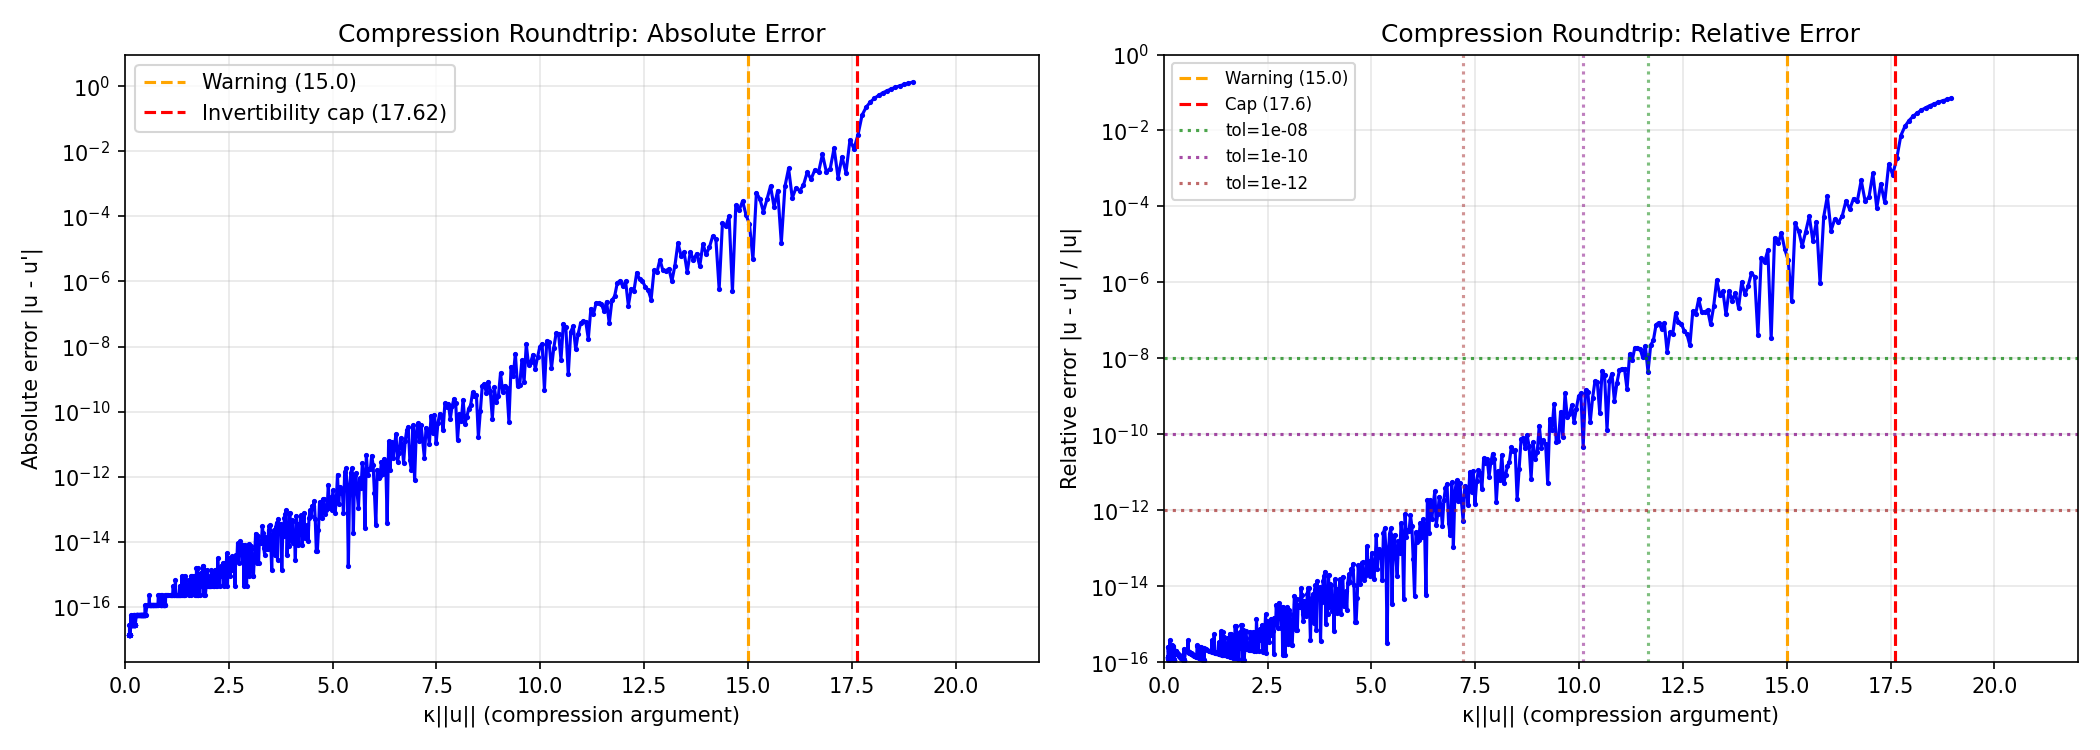
\includegraphics[width=0.99\textwidth]{roundtrip_error_profile.png}
\caption{Compression roundtrip error as a function of $\kappa\norm{u}$. Error remains below $10^{-8}$ for $\kappa\norm{u} < 11.7$. Degradation becomes noticeable beyond $\kappa\norm{u} \approx 15$ and grows rapidly as the invertibility cap ($\sim 17.6$) is approached.}
\label{fig:roundtrip}
\end{figure}

%-----------------------------------------------------------------------------
\subsection{Non-Surjectivity and Attainable Region}
\label{sec:exp-attainable}

To quantify the extent to which LMS positivity makes $\Phi_\theta$ non-surjective onto the Bloch disk, we use the analytic attainable-region boundary from the mathematical development above (Proposition~\ref{prop:attainable-eps0}; see also Corollary~\ref{cor:attainable-epspos}) to compute the maximal pre-compression radius $\norm{u_{\max}(\phi)}$ along each hue direction $\phi$ (720 angles). We then map this to a disk radius
\[
 r(\phi) = \tanh\bigl(\kappa\norm{u_{\max}(\phi)}\bigr)
\]
and estimate area fraction via polar integration:
\begin{equation}
\text{Area fraction} = \frac{1}{\pi} \cdot \frac{1}{2} \int_0^{2\pi} r(\phi)^2 \, d\phi.
\end{equation}
We cross-validate with grid counting on a $100 \times 100$ polar grid. With D65-calibrated parameters ($\gamma_{LM} = 0.9589$, $\beta = 0.5474$, $\kappa = 1$):
\begin{itemize}
    \item Area fraction (polar): 0.6115
    \item Area fraction (grid): 0.6128
    \item Discrepancy: 0.0012
    \item Max $\norm{v}$ varies by hue: $\sim 0.50$ (yellow) to $\approx R_{\max}$ (approaches boundary in blue direction)
\end{itemize}

\begin{figure}[H]
\centering
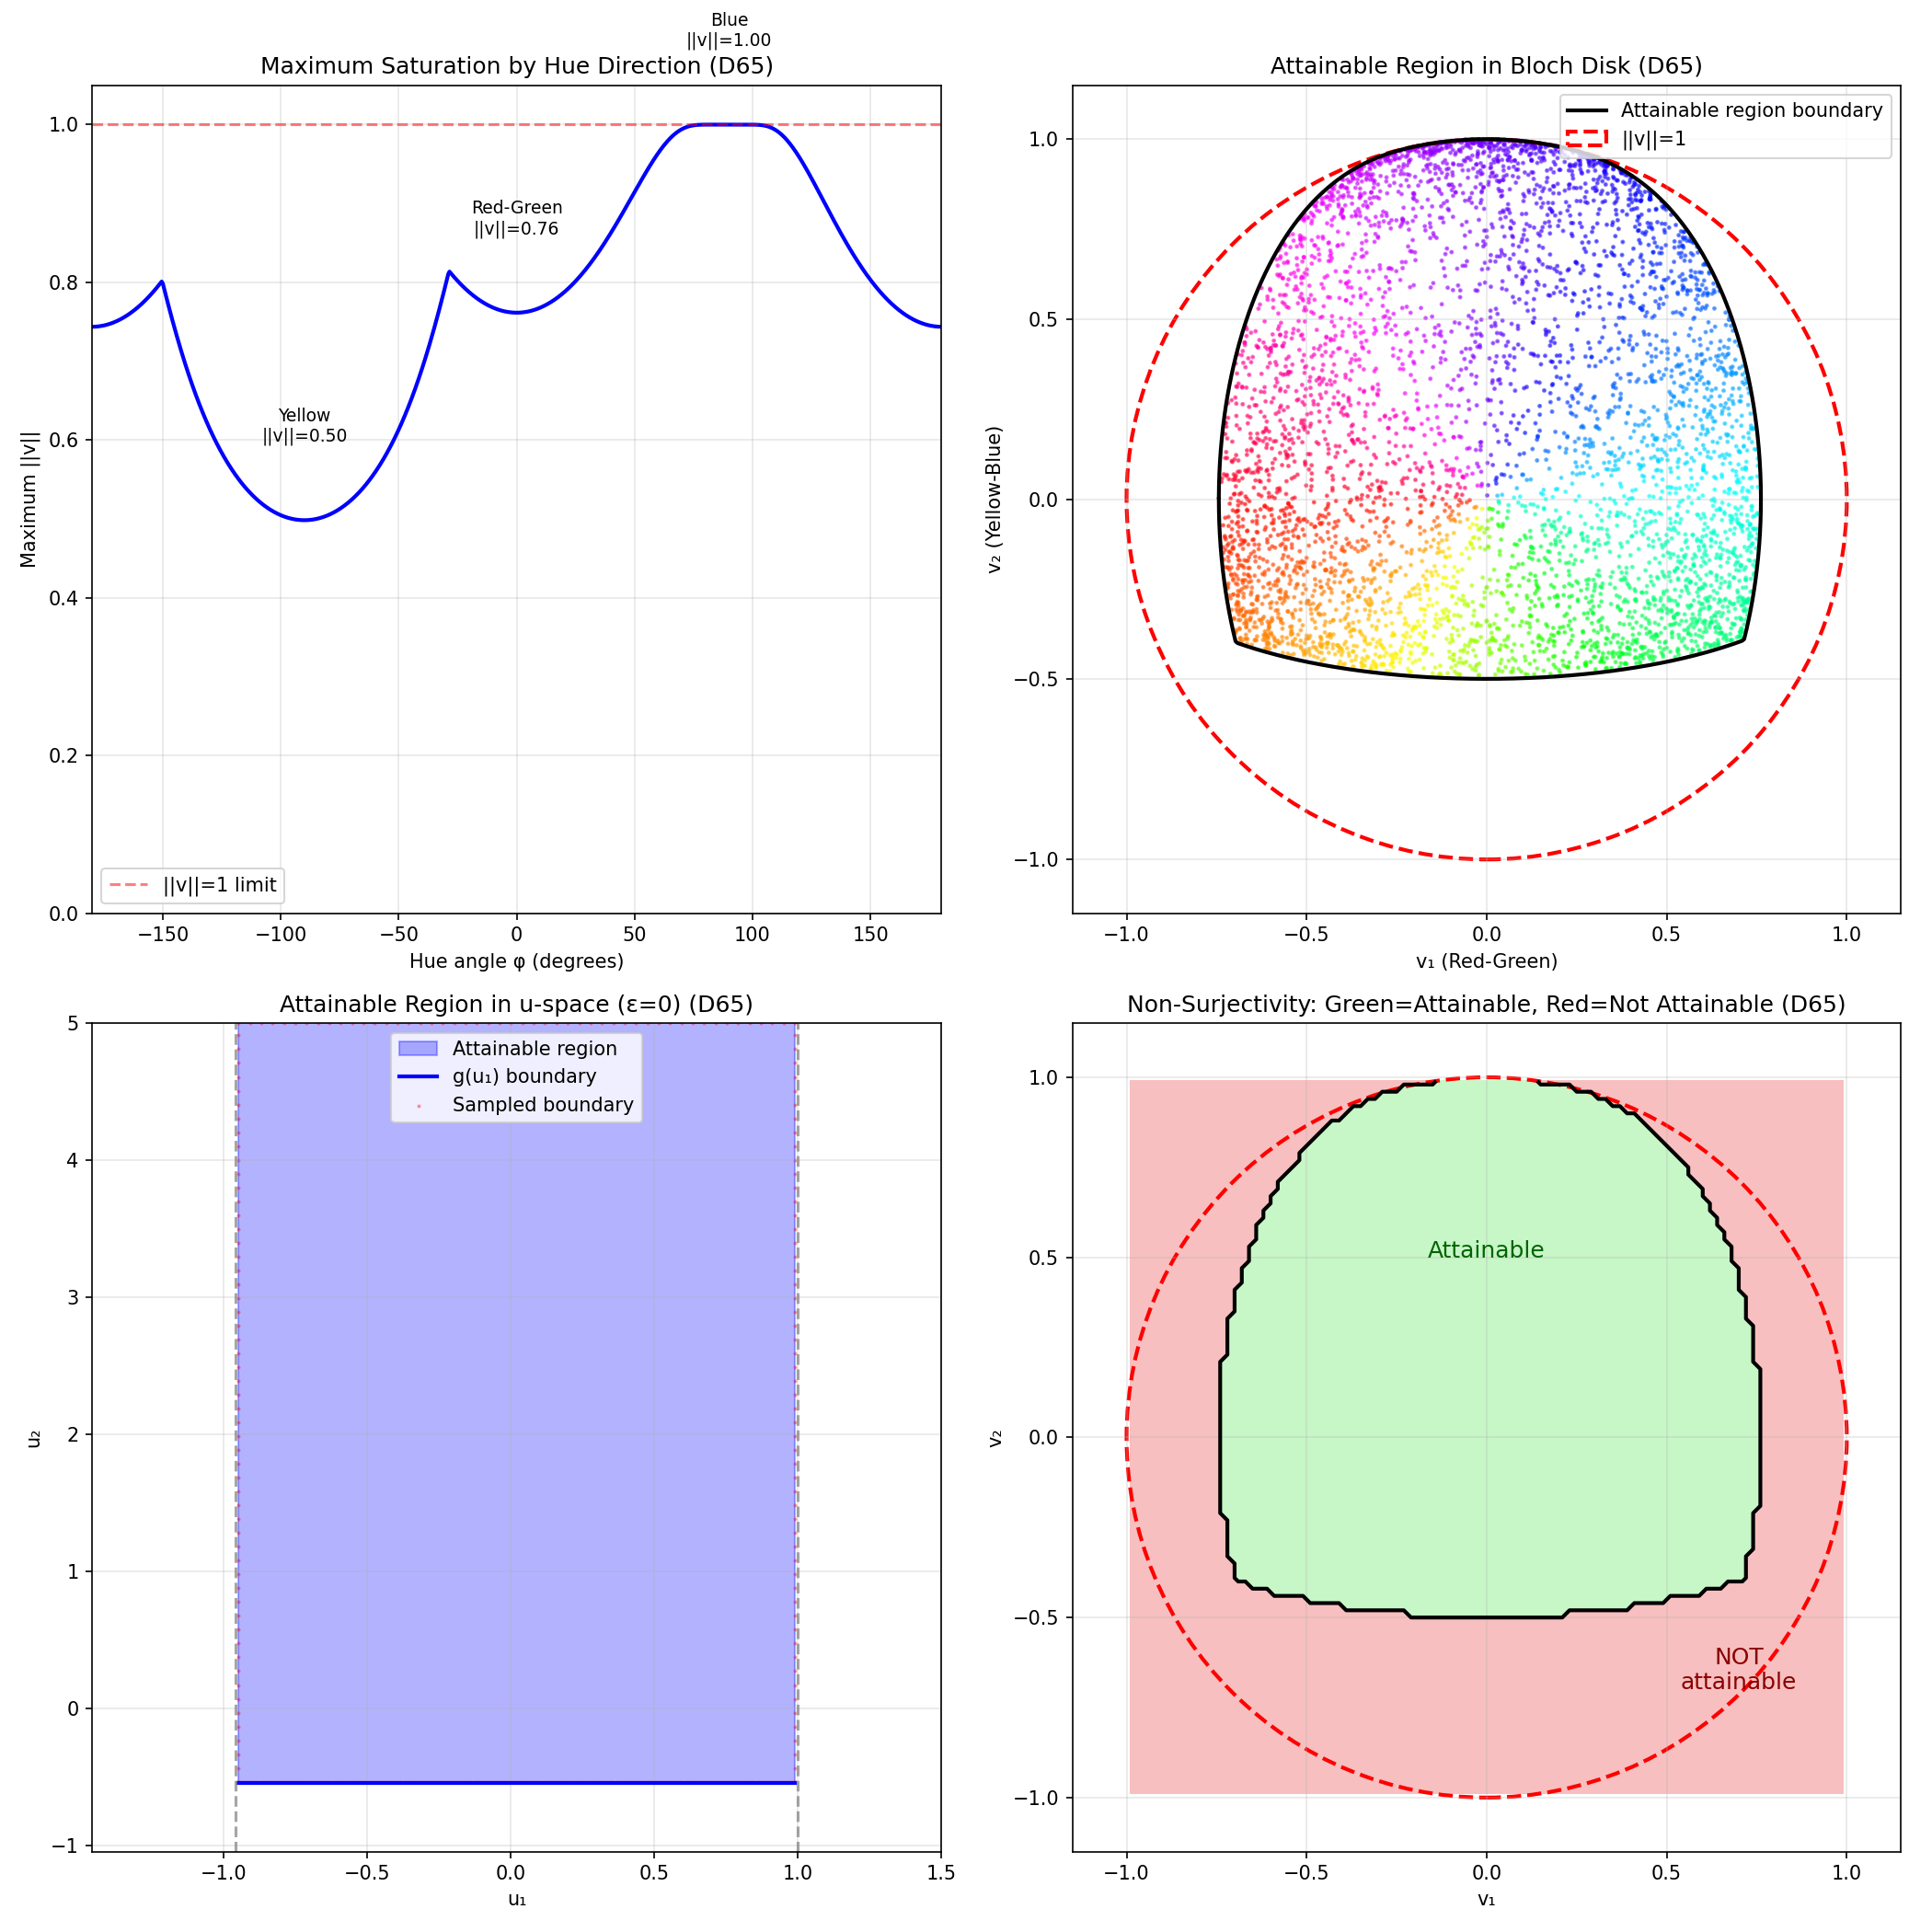
\includegraphics[width=0.85\textwidth]{gamut_boundary_analysis.png}
\caption{Attainable region $\Phi_\theta(\mathcal{L})$ in the Bloch disk (D65-calibrated $\theta$, $\kappa=1$). The boundary curve shows max $\norm{v}$ as a function of hue angle. This boundary is computed using the closed-form $\varepsilon = 0$ expression; for fixed $\varepsilon > 0$ it coincides with the supremal boundary over all positive scalings (high-luminance limit), by the scaling relation in Proposition~\ref{prop:scale-invariance}.}
\label{fig:attainable}
\end{figure}

\paragraph{$\kappa$-dependence.} The area fraction depends on $\kappa$: increasing $\kappa$ increases radial saturation and disk occupancy. Table~\ref{tab:kappa-area} shows the effect for D65 calibration. Table values were computed using the same $r(\phi)$ discretization (720 angles) and polar integration method described above.

\begin{table}[h]
\centering
\caption{Area fraction of attainable region vs.\ compression gain $\kappa$ (D65-calibrated $\theta$).}
\label{tab:kappa-area}
\begin{tabular}{@{}cc@{}}
\toprule
$\kappa$ & Area fraction \\
\midrule
0.5 & 0.38 \\
1.0 & 0.61 \\
2.0 & 0.82 \\
\bottomrule
\end{tabular}
\end{table}

As $\kappa \to \infty$, the area fraction approaches 1, but surjectivity is not achieved for any finite $\kappa$.

In this construction, LMS positivity imposes explicit bounds on the projected chromaticity coordinates $u$, and therefore $\Phi_\theta$ cannot be surjective onto the full disk. The unreachable region ($\sim 39\%$ for $\kappa = 1$) reflects this fundamental geometric constraint, not numerical limitations.

We use \emph{area fraction} to denote the proportion of $\D$ occupied by $\Phi_\theta(\mathcal{L})$. This should be distinguished from both the footprint of a particular display gamut within $\D$ and the fraction of numerical samples that avoid saturation.

%-----------------------------------------------------------------------------
\subsection{Klein Metric Structure}
\label{sec:exp-ellipses}

To examine the non-uniform local discrimination structure predicted by the Klein geometry, and in particular its increased sensitivity near the boundary, we sample a $7 \times 7$ grid with $\norm{v} < 0.9$ and, using the Klein metric from Section~\ref{sec:geometry}, visualize unit metric ellipses (directions where $ds^2 = 1$).

\begin{figure}[ht]
\centering
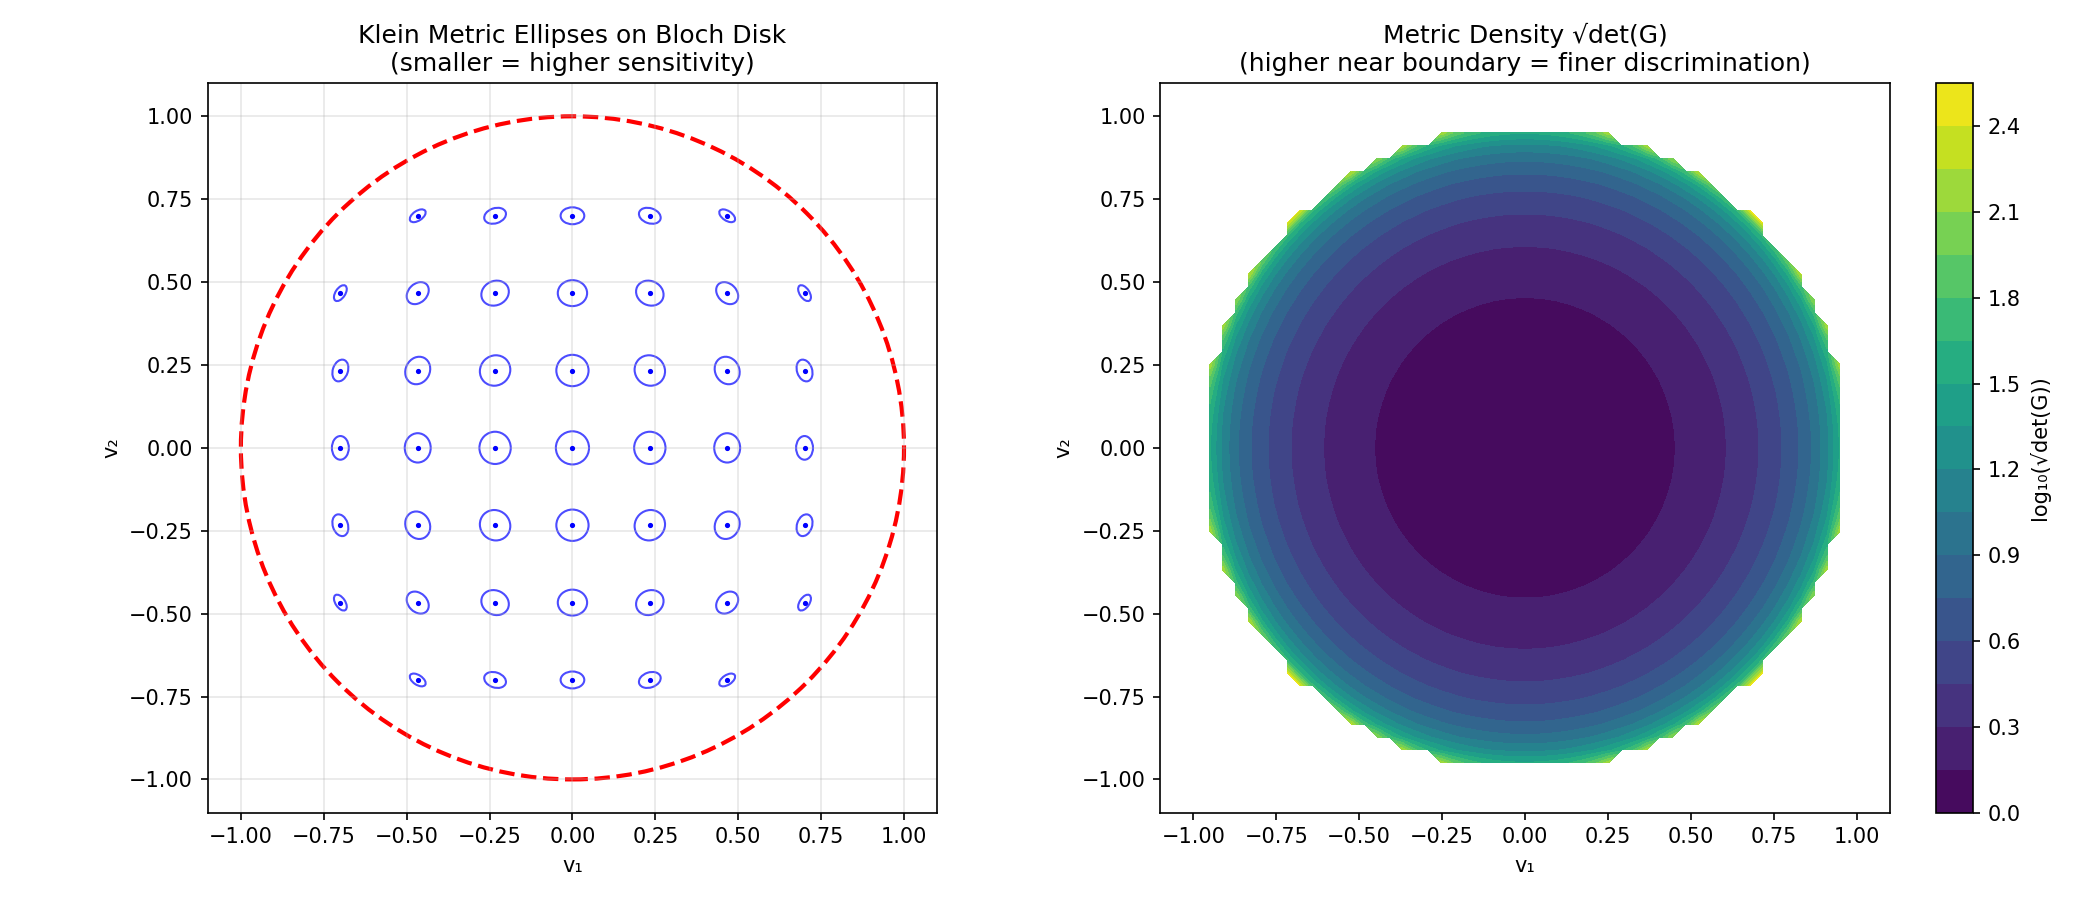
\includegraphics[width=0.99\textwidth]{discrimination_ellipses.png}
\caption{Klein metric structure on the Bloch disk. Unit metric ellipses shrink near the boundary, indicating increased sensitivity within this geometric model.}
\label{fig:ellipses}
\end{figure}

At the origin, the metric is Euclidean (circular ellipses). Near the boundary, ellipses shrink as $\sqrt{\det(G)} = (1-\norm{v}^2)^{-3/2}$ diverges: at $\norm{v} = 0.9$, this factor is $\approx 12\times$ larger than at the origin; at $\norm{v} = 0.99$, it exceeds $350\times$. Within the Klein metric geometry, equal metric steps correspond to smaller Euclidean displacements near the boundary, suggesting increased sensitivity in that region. This is a model-internal prediction that could be tested against psychophysical discrimination data in future empirical work; it does not constitute a psychophysical claim.

%-----------------------------------------------------------------------------
\subsection{Comparison with Quantum Distances}
\label{sec:exp-distances}

To compare the Hilbert geometry developed in the mathematical sections above with standard quantum information-theoretic distances on the induced rebit density family, we sample 500 random point pairs (uniform in polar, $r \in [0.1, 0.9]$, seed=42) and compute Hilbert, trace~\cite{NielsenChuang}, Bures distance, Bures angle, and Euclidean distances. Pearson and Spearman correlations provide a descriptive measure of agreement; they are not interpreted as evidence of metric equivalence.

\begin{figure}[H]
\centering
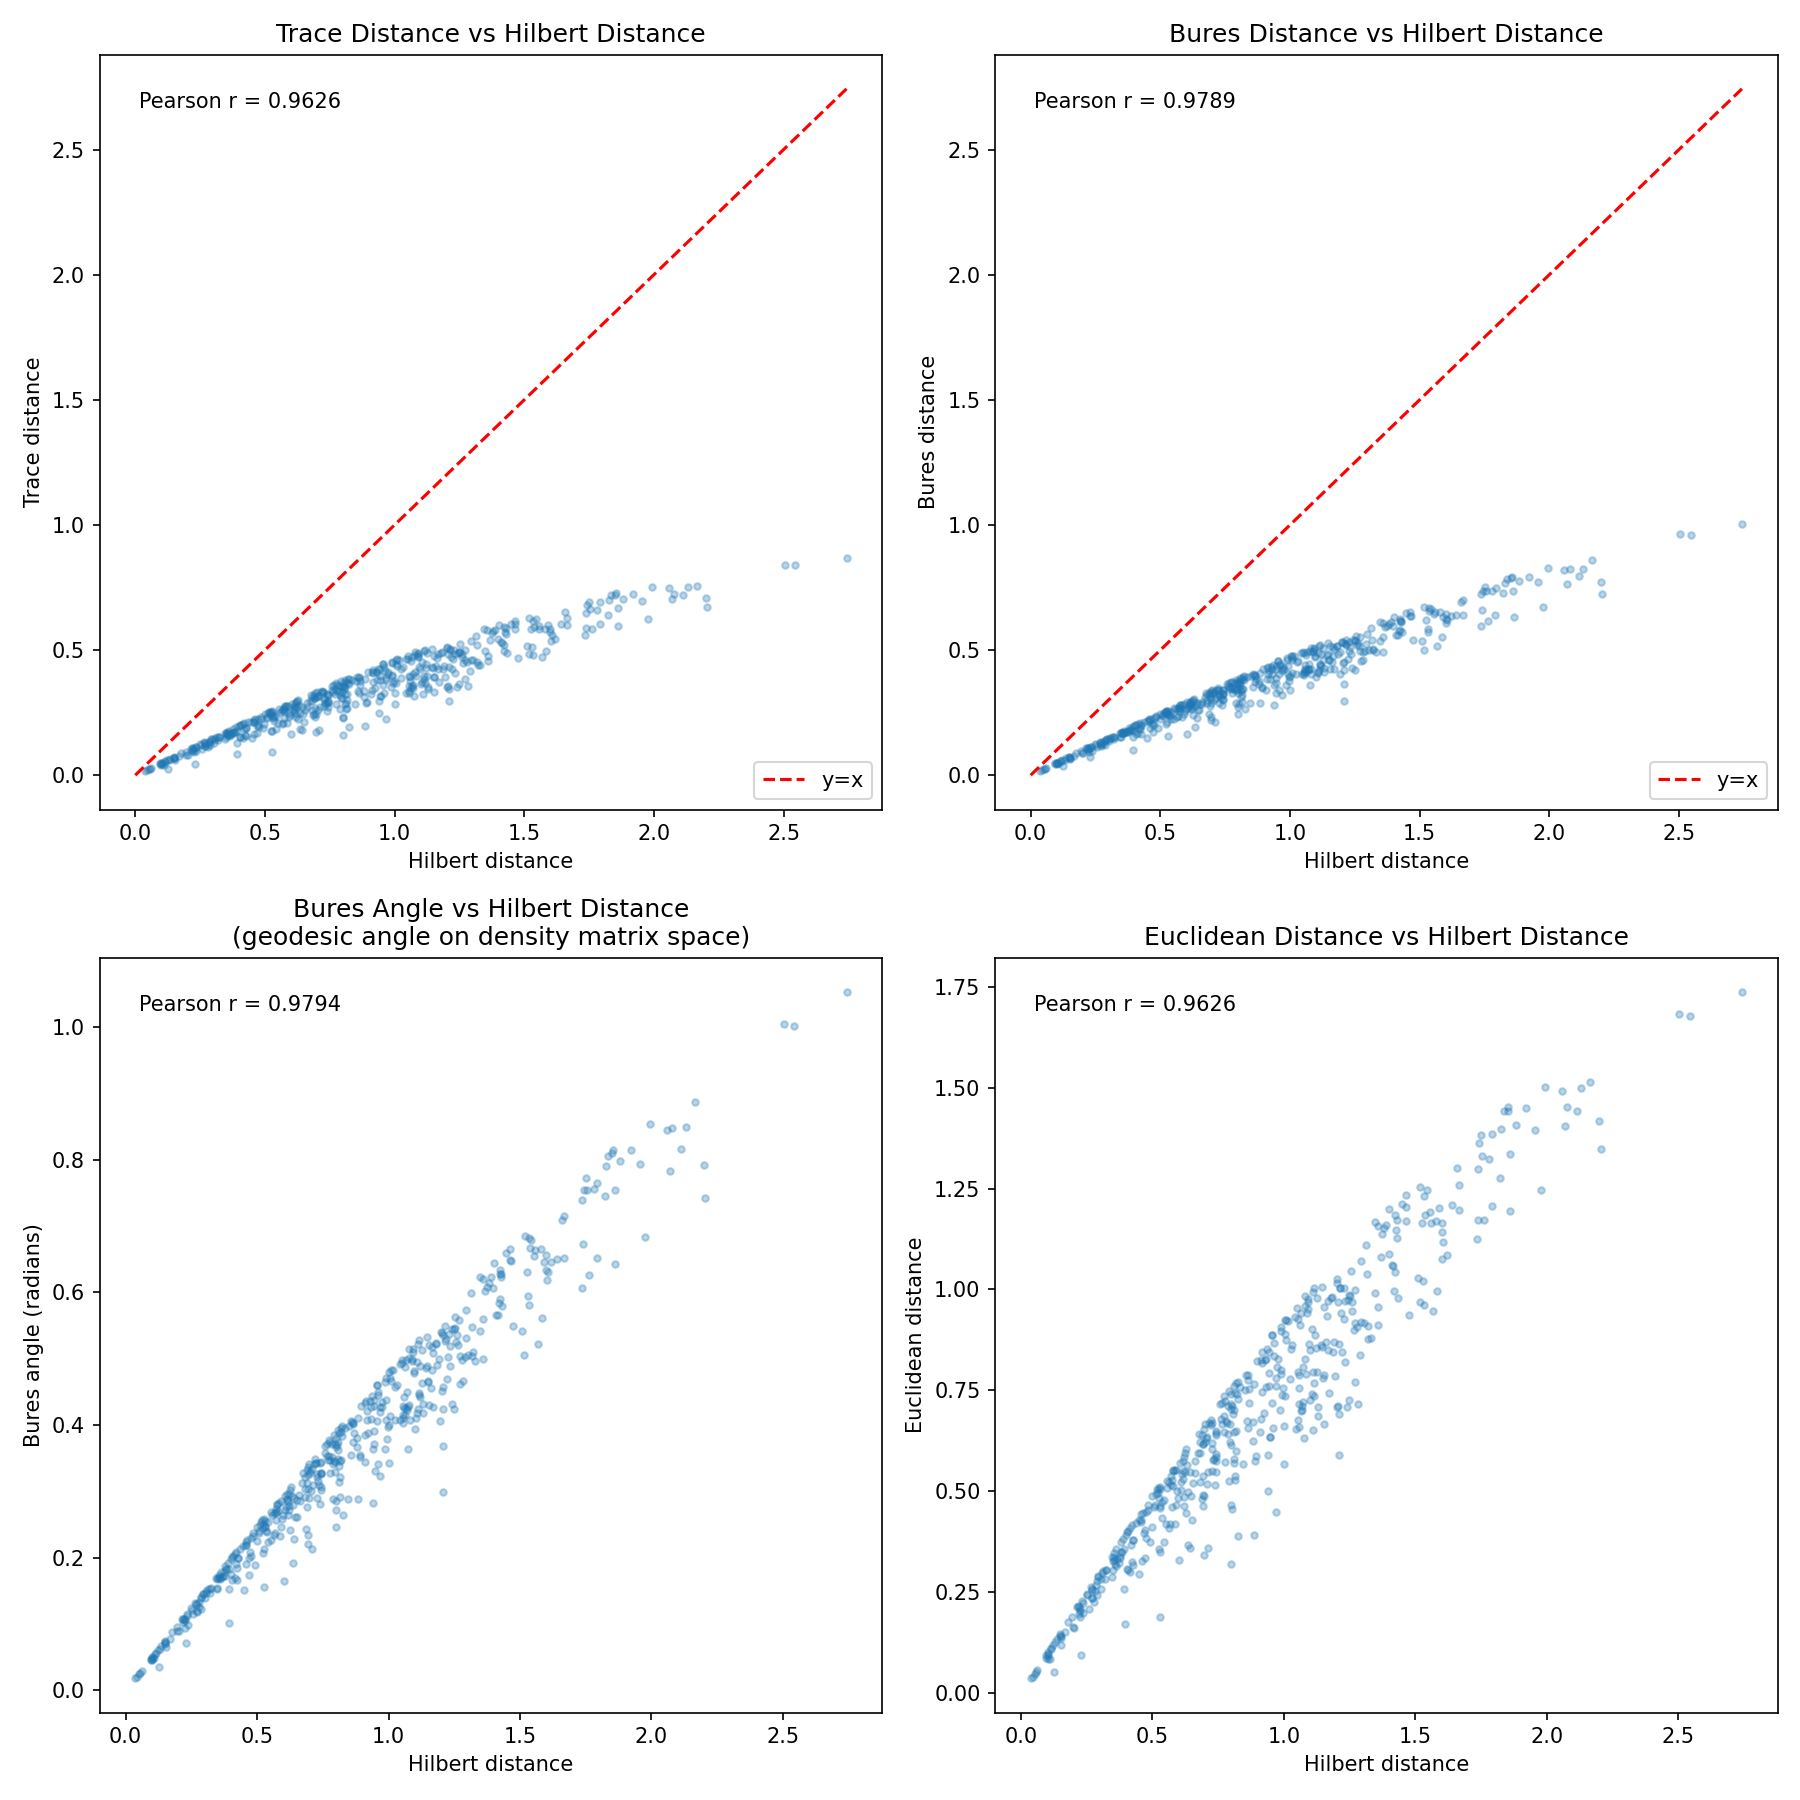
\includegraphics[width=0.85\textwidth]{distance_comparison.png}
\caption{Correlation of quantum distance measures with Hilbert distance on 500 random point pairs.}
\label{fig:distances}
\end{figure}


\begin{table}[h]
\centering
\caption{Correlation of quantum distances with Hilbert distance.}
\label{tab:correlations}
\begin{tabular}{@{}lcc@{}}
\toprule
\textbf{Distance} & \textbf{Pearson $r$} & \textbf{Spearman $r$} \\
\midrule
Trace & 0.963 & 0.956 \\
Bures & 0.979 & 0.978 \\
Bures angle & 0.979 & 0.978 \\
Euclidean & 0.963 & 0.956 \\
\bottomrule
\end{tabular}
\end{table}

As expected, the rebit trace-distance identity $D_{\text{trace}}(\rho(v_1), \rho(v_2)) = \frac{1}{2}\norm{v_1 - v_2}$ implies matching trace/Euclidean correlations. Bures distance and Bures angle (monotone transforms of fidelity) have matching Spearman correlations. All quantum distances correlate strongly with Hilbert distance ($r > 0.96$), with Bures metrics tracking most closely ($r \approx 0.98$). This comparison is descriptive on the chosen sampling distribution and does not imply metric equivalence. The strong correlations suggest the Hilbert geometry is broadly consistent with information-geometric distances on the induced density family, supporting the coherence of the rebit embedding.

%-----------------------------------------------------------------------------
\subsection{Operating Ranges for Standard Color Spaces}
\label{sec:exp-gamut}

To characterize the range of pre-compression radii induced by standard RGB color spaces, we sample $25^3 = 15625$ RGB grid points for sRGB, Display P3, and Rec.2020. Here ``Display P3'' denotes the D65, sRGB-transfer-function RGB space based on P3 primaries~\cite{DisplayP3}, not the theatrical DCI-P3 projector standard of SMPTE RP~431-2~\cite{SMPTE4312}. RGB values are sampled in linear-light coordinates in $[0,1]^3$ and converted to XYZ using standard published RGB$\to$XYZ matrices~\cite{sRGB-IEC,DisplayP3,BT2020}, then to LMS using HPE. We then compute $\norm{u}$ statistics under D65-calibrated $\theta$.

\begin{figure}[H]
\centering
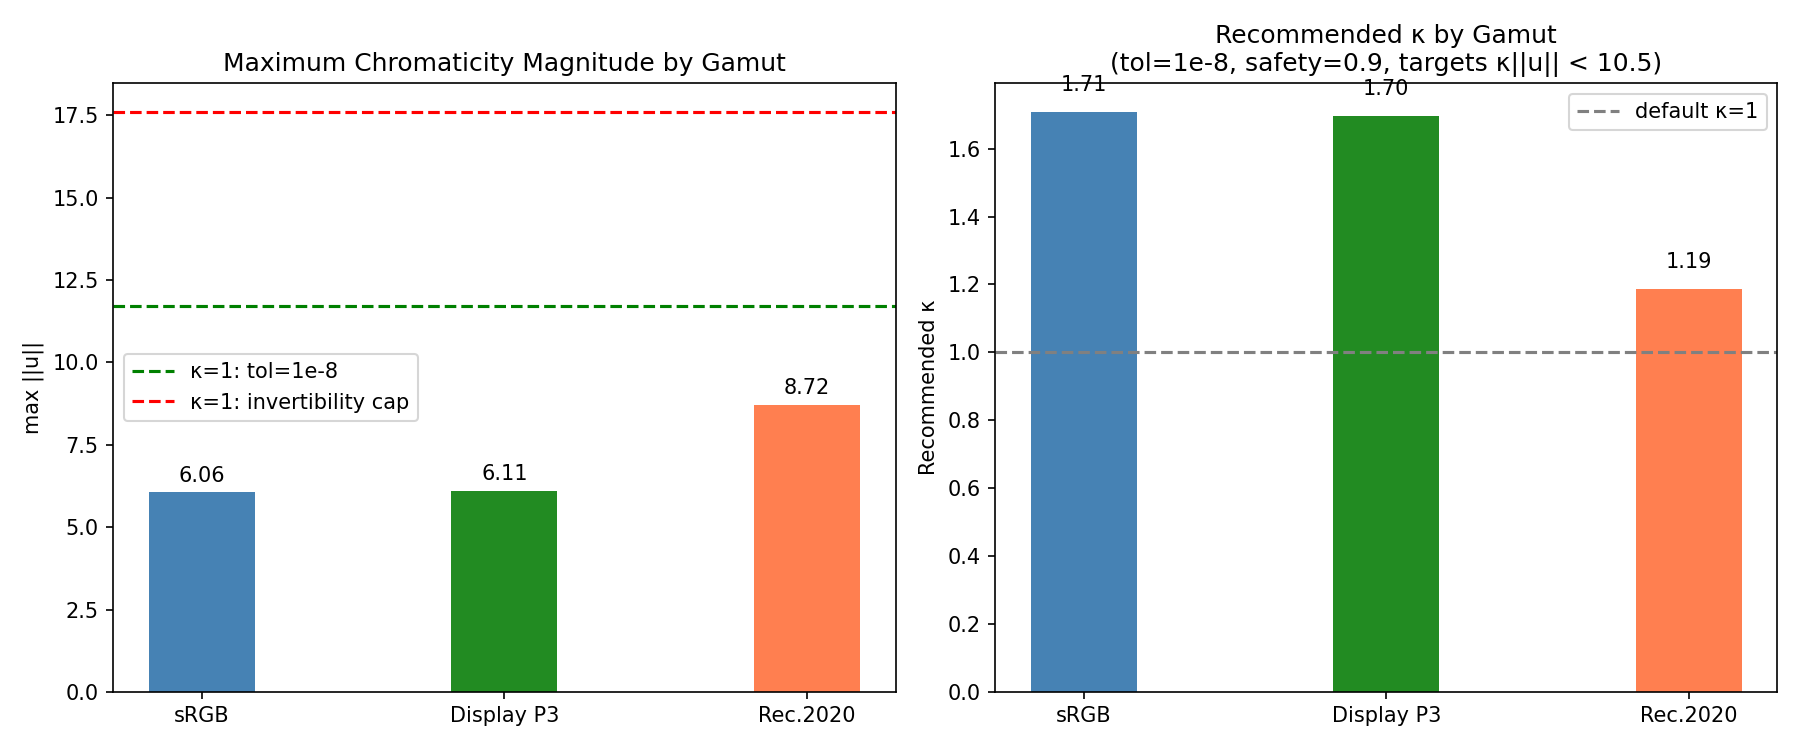
\includegraphics[width=0.85\textwidth]{gamut_comparison.png}
\caption{Display gamut footprints mapped to the Bloch disk (sRGB, Display P3, Rec.2020).}
\label{fig:gamut}
\end{figure}

\begin{table}[h]
\centering
\caption{Gamut analysis for standard color spaces (D65-calibrated $\theta$).}
\label{tab:gamut}
\begin{tabular}{@{}lccl@{}}
\toprule
\textbf{Color Space} & \textbf{Max $\norm{u}$} & \textbf{Recommended $\kappa$} & \textbf{Target} \\
\midrule
sRGB & 6.1 & 1.7 & tol $= 10^{-8}$ \\
Display P3 & 6.1 & 1.7 & tol $= 10^{-8}$ \\
Rec.2020 & 8.7 & 1.2 & tol $= 10^{-8}$ \\
\bottomrule
\end{tabular}
\end{table}

We choose $\kappa$ so that $\kappa \max\norm{u}$ stays below $0.9 \, x_{\text{tol}}$, where $x_{\text{tol}}$ is the threshold from Table~\ref{tab:precision} for the desired tolerance. For tol $= 10^{-8}$, $x_{\text{tol}} \approx 11.7$. With $\kappa = 1$, all three gamuts lie deep in the high-precision regime ($\max\norm{u} < 9$, well below the $10^{-8}$ threshold at 11.7). The recommended $\kappa$ values in Table~\ref{tab:gamut} are the largest gains that still keep $\kappa \max\norm{u}$ below the $10^{-8}$ precision threshold (with a 10\% safety factor), allowing fuller use of the disk without entering saturation-prone regimes. For more conservative, precision-critical settings, smaller $\kappa$ provides larger numerical margin.

%-----------------------------------------------------------------------------
\subsection{Image-Space Decomposition}
\label{sec:exp-image}

To examine how the construction behaves in an image-processing setting, we apply $\Phi_\theta$ to both synthetic sanity-check images and a small real-image corpus. The full pipeline is sRGB $\to$ linearize (EOTF) $\to$ XYZ $\to$ LMS (HPE) $\to$ $\Phi_\theta$ (image mode, $\varepsilon = 0.01$). We then extract hue $= \operatorname{atan2}(v_2, v_1)$, Bloch radius $\norm{v}$, entropy $S(\rho(v))$, and entropy-based saturation $\Sigma=1-S(\rho(v))$.

\begin{figure}[H]
\centering
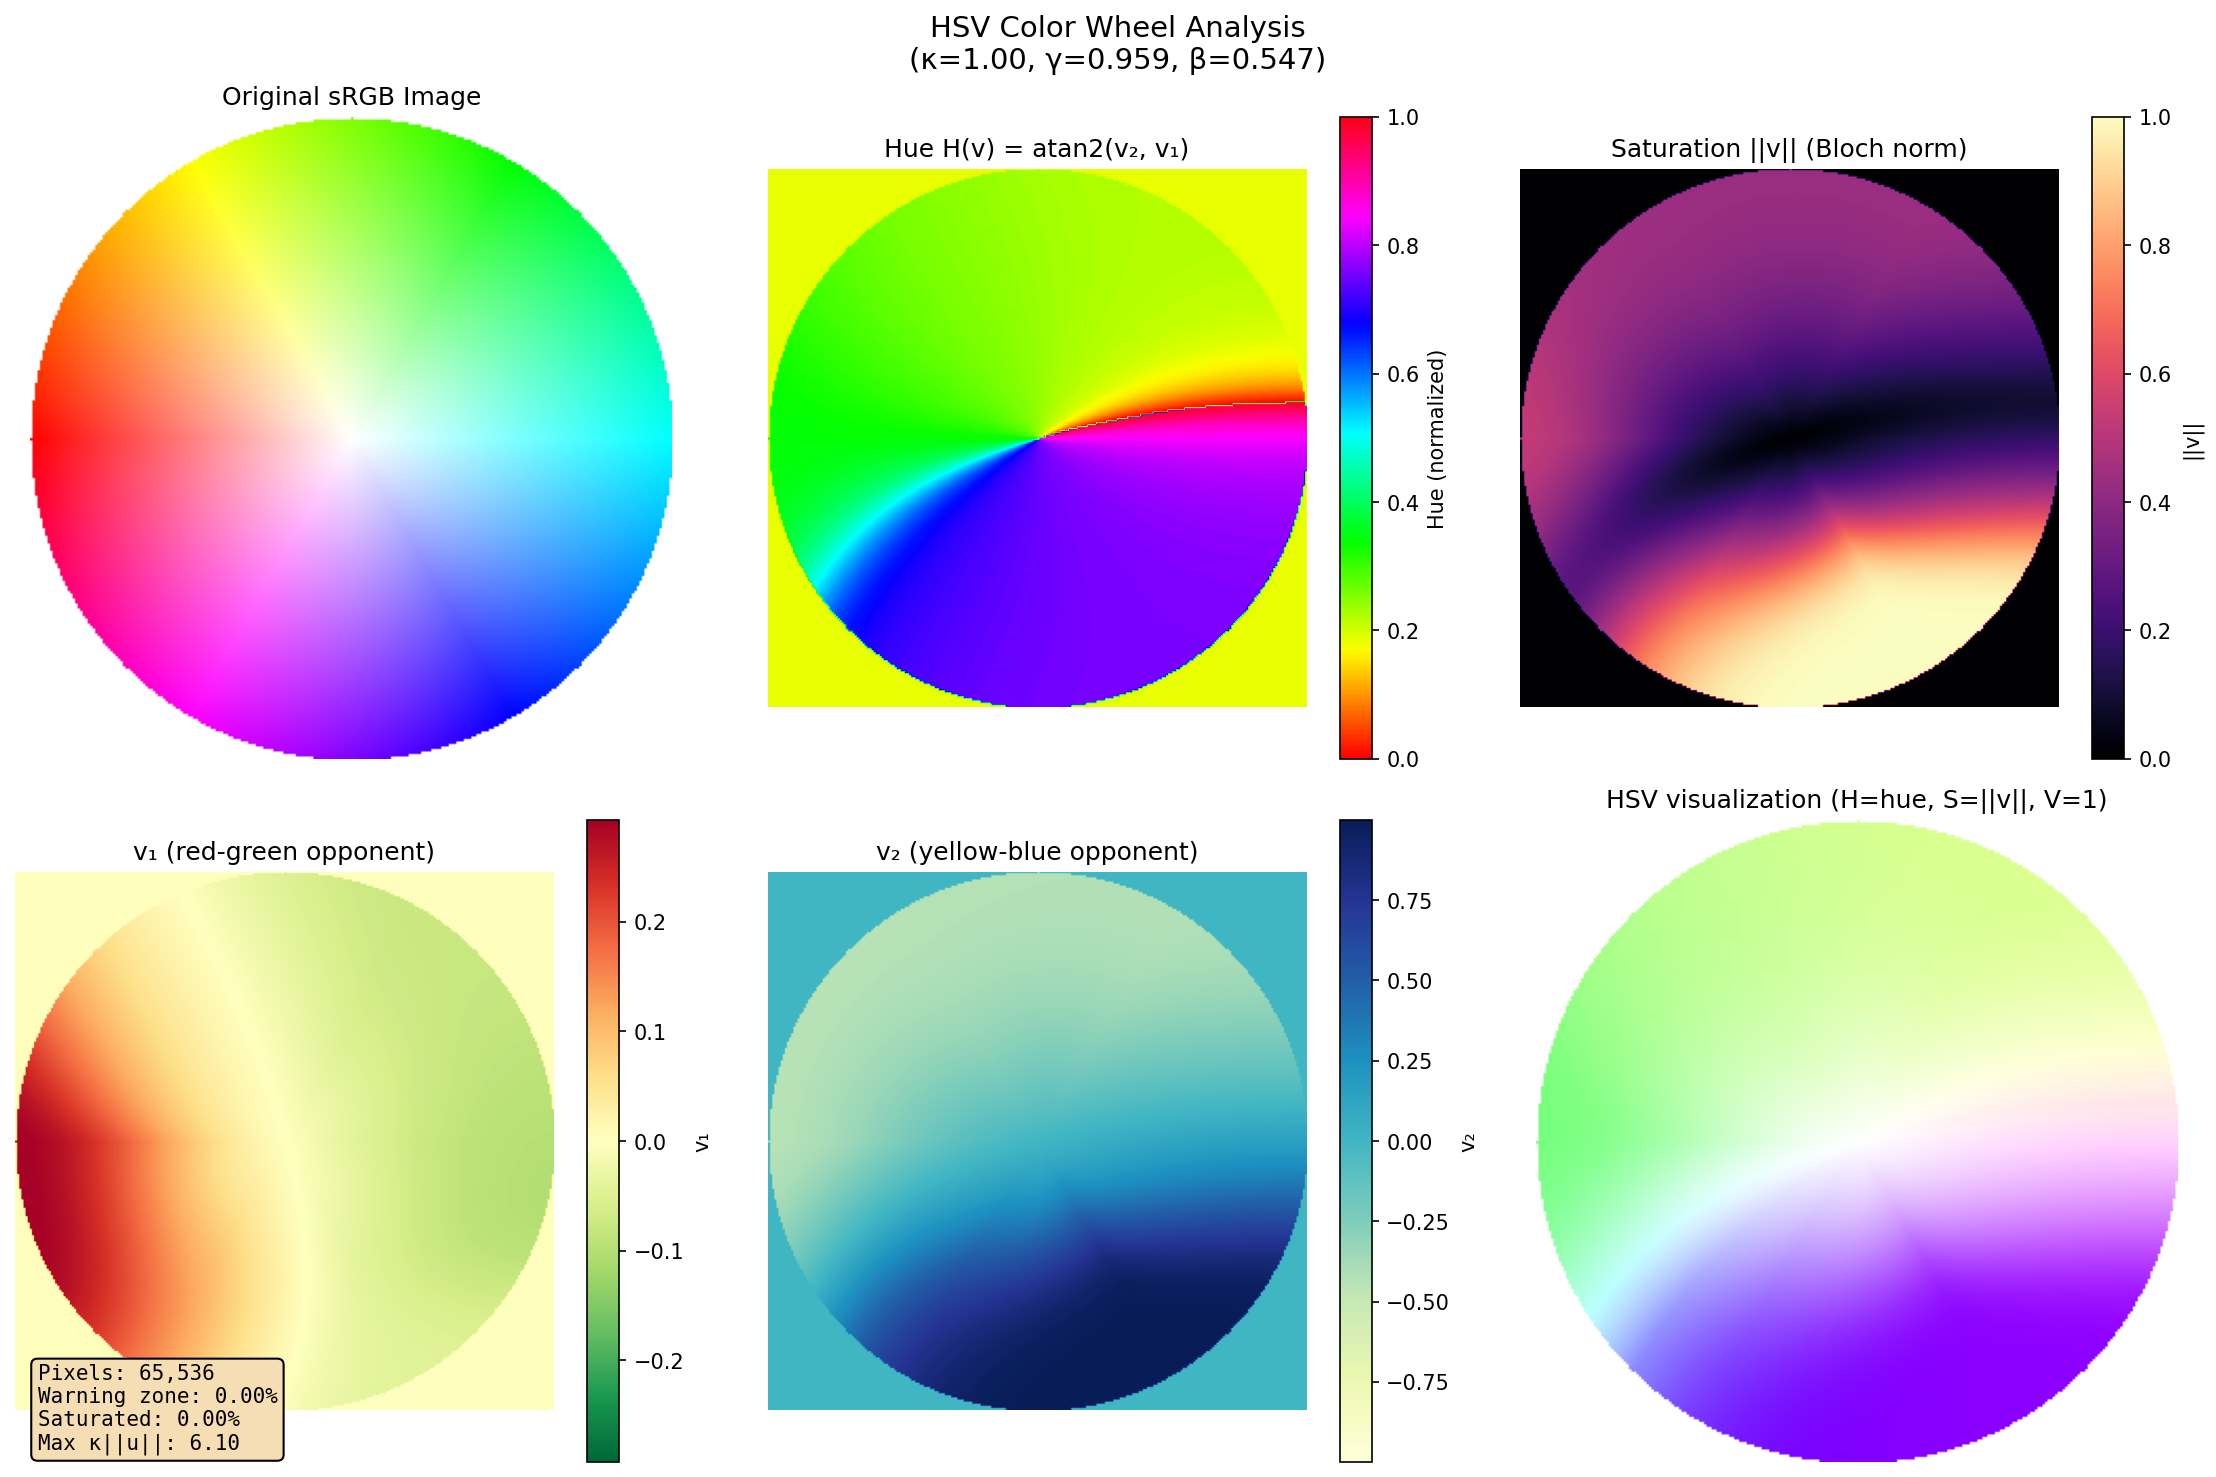
\includegraphics[width=0.99\textwidth]{image_demo_hsv_wheel.png}
\caption{Synthetic sanity check: original RGB (left), extracted hue (center), and entropy-based saturation (right).}
\label{fig:image-demo}
\end{figure}

Hue varies smoothly around the color wheel, confirming coherent opponent encoding in image space. Saturation peaks at fully saturated colors and drops to zero at white and gray, as expected.

We then process three public sample photographs (astronaut, coffee, rocket) from the scikit-image sample-image repository, resized to at most $320$ pixels on the long side. The run contains $239{,}040$ pixels. Across the corpus, the maximum pre-compression radius is $\max\norm{u}=2.197$, the maximum Bloch radius is $\max\norm{v}=0.976$, the compression warning fraction is $0$, and the maximum sRGB reconstruction RMSE after luminance-conditioned inversion is $1.95\times 10^{-16}$. Thus, for ordinary photographic content, the mapping remains far inside the numerical precision regimes identified in Table~\ref{tab:precision}.

\begin{figure}[H]
\centering

\includegraphics[width=0.99\textwidth]{real_image_benchmark_examples.png}
\caption{Real-image corpus examples. Each image is mapped through sRGB $\to$ XYZ $\to$ LMS $\to \Phi_\theta$ and visualized by hue, entropy-based saturation, and Bloch coordinate channels.}
\label{fig:real-image-examples}
\end{figure}

\begin{figure}[H]
\centering

\includegraphics[width=0.99\textwidth]{real_image_benchmark_summary.png}
\caption{Real-image benchmark summary for the public sample corpus. The benchmark records per-image distributions of $\norm{u}$ and $\norm{v}$, compression safety margin relative to empirical roundtrip thresholds, and Bloch-disk pixel samples. Warning and saturation fractions are zero for this run.}
\label{fig:real-image-summary}
\end{figure}

\begin{table}[H]
\centering
\caption{Real-image corpus benchmark (D65-calibrated $\theta$, HPE LMS, $\kappa=1$, $\varepsilon=0.01$).}
\label{tab:real-image-benchmark}
\begin{tabular}{@{}lrrrr@{}}
\toprule
\textbf{Image} & \textbf{Pixels} & $\max\norm{u}$ & $\max\norm{v}$ & \textbf{RGB RMSE} \\
\midrule
Astronaut & 102400 & 2.197 & 0.976 & $1.9\times 10^{-16}$ \\
Coffee & 68160 & 0.558 & 0.507 & $1.7\times 10^{-16}$ \\
Rocket & 68480 & 0.997 & 0.760 & $1.4\times 10^{-16}$ \\
\bottomrule
\end{tabular}
\end{table}

%-----------------------------------------------------------------------------
\subsection{Bloch-Domain Image Operations}
\label{sec:exp-image-operations}

The Bloch representation also supports image operations that are native to the disk geometry. We implement three operations on real sample images: hyperbolic-radius saturation scaling, Klein-geodesic image blending, and relative chromatic adaptation by gyrotranslation. In saturation scaling, hue direction in $v$ is preserved while the hyperbolic radius $\arctanh\norm{v}$ is multiplied and then mapped back to the disk. In geodesic blending, corresponding pixels are interpolated along Euclidean chords in the Klein model. In relative adaptation, an estimated bright low-saturation white point $v_w$ is removed by $(-v_w)\oplus v$ before luminance-conditioned reconstruction.

\begin{figure}[H]
\centering

\includegraphics[width=0.99\textwidth]{bloch_saturation_operation.png}
\caption{Bloch-domain saturation scaling compared with HSV and direct RGB baselines. The top row shows the processed images; the bottom row shows mean absolute RGB change from the original. The Bloch operation preserves disk hue direction and changes hyperbolic radius before reconstructing with the original luminance.}
\label{fig:bloch-saturation}
\end{figure}

\begin{figure}[H]
\centering

\includegraphics[width=0.99\textwidth]{bloch_geodesic_blend.png}
\caption{Klein-geodesic blend between two real images. In the Klein model, geodesics are Euclidean chords, so linear interpolation in $v$ follows the correct unparameterized geodesic.}
\label{fig:bloch-blend}
\end{figure}

\begin{figure}[H]
\centering

\includegraphics[width=0.99\textwidth]{bloch_relative_adaptation_comparison.png}
\caption{Relative chromatic adaptation via Klein gyrotranslation by the estimated image white point. This is an algebraic color-constancy operation in the model coordinates, not a claim of human adaptation equivalence.}
\label{fig:bloch-adaptation}
\end{figure}

These experiments demonstrate that $\Phi_\theta$ is not only a coordinate visualization: disk-domain operations can be composed with the inverse map to produce concrete RGB images. The output JSON records gamut clipping, estimated white point, and operation parameters for auditability.

%-----------------------------------------------------------------------------
\subsection{Induced Sensitivity in LMS Space}
\label{sec:exp-sensitivity}

To characterize the spatially varying sensitivity induced in LMS space by the pullback of the Klein geometry, we create a $30 \times 30$ grid in sRGB space ($R$, $B$ varied, $G = 0.5$ fixed), convert to LMS, and compute the Jacobian Frobenius norm $\fnorm{J_{\Phi_\theta}}$ and pullback metric trace $\operatorname{Tr}(G_{\mathrm{LMS}})$.

\begin{figure}[H]
\centering
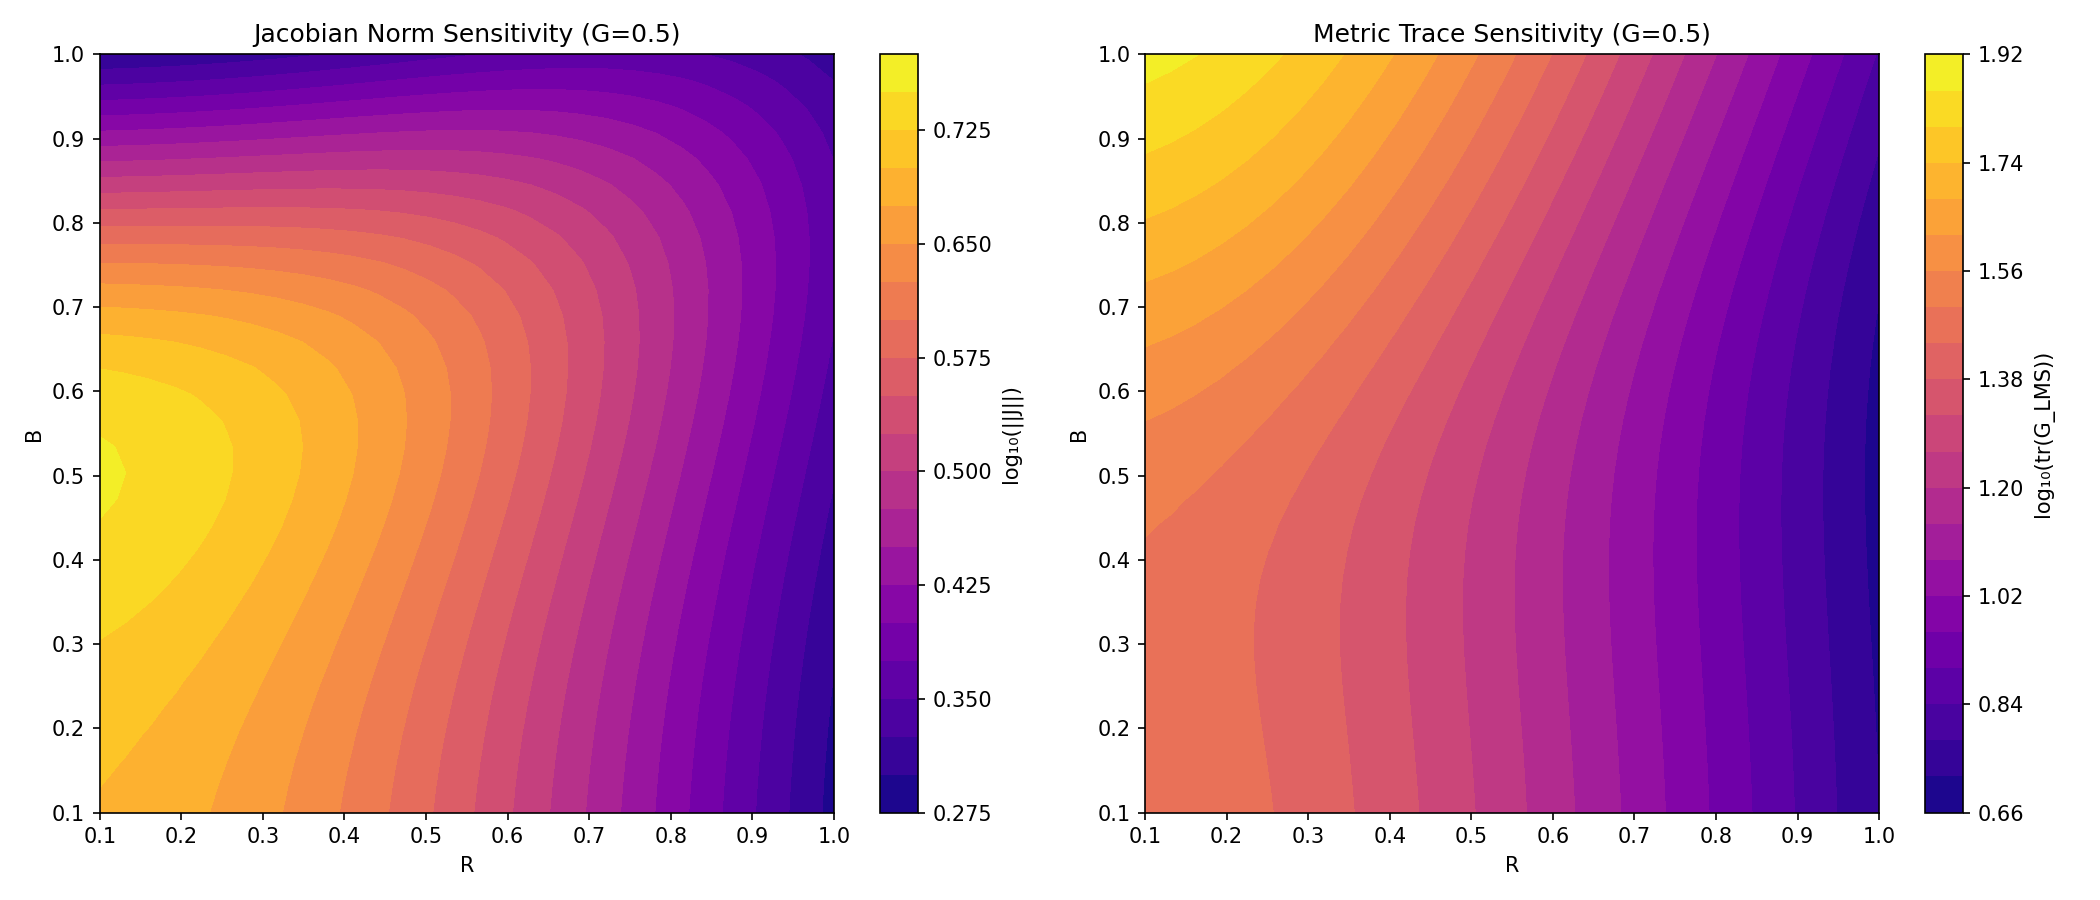
\includegraphics[width=0.85\textwidth]{sensitivity_heatmap.png}
\caption{Sensitivity heatmap: Jacobian norm (left) and pullback metric trace (right) across LMS input space.}
\label{fig:sensitivity}
\end{figure}

Jacobian norm ranges from $\sim 2.0$ to $\sim 5.7$; metric trace ranges from $\sim 5$ to $\sim 76$. Regions with large $\operatorname{Tr}(G_{\mathrm{LMS}})$ indicate strong amplification of LMS perturbations in disk coordinates. These correspond to colors near the attainable region boundary, consistent with the divergent metric behavior predicted by the Klein geometry. Here ``sensitivity'' refers to differential amplification in model coordinates, not to measured JND sensitivity.

%-----------------------------------------------------------------------------
\subsection{Parameter and Conversion Ablations}
\label{sec:exp-ablation}

We next perform a formal ablation over the choices most likely to affect practical use: compression gain $\kappa$, luminance floor $\varepsilon$, RGB gamut, XYZ$\to$LMS matrix, and whitepoint calibration mode. The ablation samples an $11^3$ RGB grid for sRGB, Display~P3, and Rec.~2020, evaluates HPE, CAT02, and Bradford cone-response matrices, and records $\norm{u}$, $\norm{v}$, warning fractions, attainable area fraction, and recommended $\kappa$ for the $10^{-8}$ reconstruction-tolerance regime.

\begin{figure}[H]
\centering

\includegraphics[width=0.99\textwidth]{parameter_ablation_summary.png}
\caption{Parameter and conversion ablation. Left: maximum $\kappa\norm{u}$ across $(\kappa,\varepsilon)$ for sRGB/HPE/D65. Right: LMS-matrix sensitivity under fixed sRGB/D65 settings.}
\label{fig:parameter-ablation}
\end{figure}

\begin{table}[H]
\centering
\caption{Representative ablation rows for sRGB/D65, $\kappa=1$, $\varepsilon=0.01$.}
\label{tab:lms-matrix-ablation}
\begin{tabular}{@{}lccc@{}}
\toprule
\textbf{LMS matrix} & $\max\norm{u}$ & \textbf{Recommended $\kappa$} & \textbf{Regime at $\kappa=1$} \\
\midrule
HPE & 5.998 & 1.726 & Ultra-precise \\
Bradford & 14.973 & 0.691 & Degraded \\
CAT02 & 39.845 & 0.260 & Non-invertible without lower $\kappa$ \\
\bottomrule
\end{tabular}
\end{table}

The HPE pipeline used in the main experiments is stable at $\kappa=1$ with zero warning fraction and attainable area fraction $0.6115$. The CAT02 and Bradford rows show that the RGB$\to$LMS bridge is not an innocuous implementation detail: alternative matrices can move common display colors into much larger pre-compression radii and require substantially smaller $\kappa$ for reliable inversion. This supports treating LMS conversion as an explicit experimental factor rather than as hidden preprocessing.

%-----------------------------------------------------------------------------
\subsection{Controlled White-Balance Experiment}
\label{sec:exp-white-balance}

As a controlled image-processing task, we use an approximate ColorChecker-style sRGB patch table, convert patches to LMS, apply known synthetic diagonal LMS illuminant gains, and compare correction methods against the reference chart. Because the simulated casts are diagonal in LMS, the von~Kries diagonal correction is expected to be exact and serves as an upper baseline. We compare it with no correction, Bloch relative-state correction by gyrotranslation, and Bloch whitepoint recalibration.

\begin{figure}[H]
\centering

\includegraphics[width=0.99\textwidth]{white_balance_summary.png}
\caption{Controlled white-balance experiment on approximate ColorChecker patches under synthetic LMS illuminants. Von~Kries is exact for this synthetic diagonal task; Bloch-domain corrections reduce error but are not equivalent to diagonal LMS inversion.}
\label{fig:white-balance}
\end{figure}

\begin{table}[H]
\centering
\caption{Mean $\Delta E_{76}$ by illuminant and method.}
\label{tab:white-balance}
\begin{tabular}{@{}lrrrr@{}}
\toprule
\textbf{Illuminant} & \textbf{Uncorrected} & \textbf{Von~Kries} & \textbf{Bloch relative} & \textbf{Bloch recalibrated} \\
\midrule
Warm LMS & 24.04 & 0.00 & 11.99 & 12.23 \\
Cool LMS & 22.48 & 0.00 & 10.96 & 10.27 \\
Green LMS & 40.22 & 0.00 & 6.35 & 5.49 \\
\bottomrule
\end{tabular}
\end{table}

The result is deliberately interpreted as a computational ablation, not a claim that the Bloch operation is a better white-balance algorithm than von~Kries correction. It shows that disk-relative operations can partially compensate chromatic casts while preserving the model's geometry, and it identifies the residual error left by using a two-dimensional chromatic state rather than directly inverting the known three-channel illuminant.

%-----------------------------------------------------------------------------
\subsection{MacAdam Ellipse Calibration Pilot}
\label{sec:exp-macadam}

Finally, we run a small calibration-readiness experiment against the classic MacAdam 1942 observer-PGN ellipse table~\cite{MacAdam1942,Wyszecki1982}. We convert the $25$ ellipse centers from $xyY$ to XYZ and then to LMS, compute the local pullback metric of $\Phi_\theta$ in the $(x,y)$ chromaticity plane, and compare the predicted ellipse aspect ratio and orientation with the tabulated ellipse shapes. We fit only a small parameter subset: $\kappa$, $w_L/w_M$, and $\varepsilon$, while keeping the D65 achromatic calibration of $\gamma_{LM}$ and $\beta$.

\begin{figure}[H]
\centering

\includegraphics[width=0.99\textwidth]{psychophysical_bridge_pilot.png}
\caption{MacAdam ellipse calibration pilot. Blue ellipses show target MacAdam shapes; red dashed ellipses show the fitted pullback-metric shapes. The fit modestly improves axis-ratio error but leaves large orientation error, indicating that the present $\theta$-parameterization alone is not a full psychophysical model.}
\label{fig:macadam-pilot}
\end{figure}

\begin{table}[H]
\centering
\caption{MacAdam ellipse pilot diagnostics. The objective combines squared log axis-ratio error and squared orientation error normalized by $90^\circ$.}
\label{tab:macadam-pilot}
\begin{tabular}{@{}lccc@{}}
\toprule
\textbf{Fit} & \textbf{Objective} & \textbf{Mean angle error} & \textbf{Mean log axis-ratio error} \\
\midrule
D65 fixed & 0.686 & $60.6^\circ$ & 0.294 \\
Fit $\kappa$ & 0.630 & $63.3^\circ$ & 0.234 \\
Fit $\kappa,w_L/w_M,\varepsilon$ & 0.593 & $59.4^\circ$ & 0.244 \\
\bottomrule
\end{tabular}
\end{table}

Five-fold cross-validation of the three-parameter fit gives mean train objective $0.592$ and mean held-out objective $0.626$, so the small improvement is stable under this pilot split. The large residual orientation error is the more important result: it indicates that matching classical discrimination ellipses will likely require either additional opponent-basis freedom, an observer-specific convex domain in the disk, or the Finsler refinements suggested by the intrinsic theory, rather than merely retuning $\kappa$ and luminance weights.

%=============================================================================
\section{Discussion}
\label{sec:discussion}
%=============================================================================

The main role of the present construction is to provide an explicit bridge between the intrinsic rebit geometry of perceived chromaticity and computable cone-response coordinates. In that sense, the paper does not propose a new axiomatic geometry, but rather a concrete realization of one: a smooth map $\Phi_\theta \colon \mathcal{L} \to \mathbb{D}$ with an analytically tractable attainable region, a distinguished achromatic locus, and a luminance-conditioned inverse on its natural domain of feasibility. The numerical experiments show that this bridge can be implemented stably in float64 arithmetic over parameter ranges relevant to standard RGB gamuts and ordinary real-image content. Just as importantly, the attainable-region analysis makes clear that the failure of surjectivity is not a numerical artifact of the implementation, but a structural consequence of LMS positivity together with the chosen opponent transform and normalization.

These results should nevertheless be interpreted at the appropriate level of scope. The comparisons with trace distance, Bures distance, and Bures angle are descriptive comparisons on the induced rebit family, not evidence that any of these metrics---including the Hilbert metric itself---is a validated model of perceptual dissimilarity. Likewise, the image-space decompositions, Bloch-domain image operations, controlled white-balance experiment, and pullback-metric calculations are best read as model-internal illustrations of the geometry induced by $\Phi_\theta$. They show that the construction yields coherent opponent coordinates, entropy-based saturation, stable real-image inversion, and a pronounced amplification of perturbations near the attainable boundary, but they do not by themselves establish correspondence with discrimination thresholds, perceived hue, or perceived saturation.

A second limitation concerns calibration and modeling choices that lie outside the Jordan-algebraic framework. The passage from device or tristimulus coordinates to LMS depends on the selected cone fundamentals and adaptation transform; different XYZ$\to$LMS matrices (HPE, CAT02, Stockman--Sharpe~\cite{StockmanSharpe2000}) will in general induce different coordinates in the disk. Even within the present parameterization, fixing $\gamma_{LM}$ and $\beta$ from D65 aligns the whitepoint with the origin, but the luminance weights ($w_L$, $w_M$), luminance floor $\varepsilon$, and compression gain $\kappa$ are not inferred from psychophysical data. These parameters influence the shape of the attainable image of a device gamut, the pullback metric on LMS space, and the range on which reconstruction remains numerically reliable. Moreover, because $\Phi_\theta$ maps $\R^3$ to $\R^2$, the induced metric $G_{\mathrm{LMS}} = J^\top G_\D J$ is necessarily rank-deficient; for $\varepsilon = 0$, the overall scale direction lies in its null space. Reconstruction $\widetilde{\Phi}_\theta^{-1}(v; Y)$ may therefore fail positivity outside the attainable region at the prescribed luminance, and the practical clamp at $R_{\max} = 1 - 10^{-15}$ introduces a finite invertibility limit that is numerical rather than geometric.

Precisely because the map is explicit, these limitations also indicate a concrete research program. The MacAdam pilot shows that low-dimensional tuning of $\kappa$, $w_L/w_M$, and $\varepsilon$ gives only a modest improvement and leaves substantial ellipse-orientation error, so psychophysical agreement should not be expected from parameter retuning alone. One can now ask whether the opponent basis should be fitted, whether the attainable domain should be replaced by an observer-specific convex body, and whether the pullback or Finsler geometry predicts known phenomena such as MacAdam ellipses, surround-dependent crispening, or other context effects. More broadly, the construction provides a workable interface between physiological color coordinates, convex/projective geometry, and the rebit formalism developed by Berthier, Provenzi, and collaborators. If that formalism is to function as a model of perception rather than only as an intrinsic characterization of chromatic state space, some explicit embedding of this kind appears necessary; the present map is intended as a mathematically transparent starting point for that program.

%=============================================================================
\section{Reproducibility}
\label{sec:reproducibility}
%=============================================================================

All experiments are reproducible from the package directory via
\[
\texttt{python examples/run\_all\_figures.py --output-dir results/publishable\_run}.
\]
The runner records git commit hash when available, dirty-worktree status, Python/NumPy versions, parameter values, script command lines, script success/failure status, and SHA-256 checksums for generated PNG, JSON, and CSV artifacts. Real-image sample sources are cached under \texttt{data/sample\_images/} with a separate source manifest and per-image checksums. Scripts use deterministic sampling where randomness is present (seed $42$). The HPE matrix and D65 whitepoint (XYZ $= (0.95047, 1.0, 1.08883)$) are used throughout unless otherwise noted; scripts that ablate RGB gamut, LMS matrix, $\kappa$, $\varepsilon$, or whitepoint mode write those settings explicitly to their JSON/CSV outputs.

%=============================================================================
% End of Implementation Part
%=============================================================================

\bibliographystyle{plain}
\begin{thebibliography}{99}

\bibitem{Newton1704}
I.~Newton.
\newblock \emph{Opticks, or, A Treatise of the Reflections, Refractions, Inflections and Colours of Light}.
\newblock London, 1704.

\bibitem{Grassmann1853}
H.G.~Grassmann.
\newblock Zur Theorie der Farbenmischung.
\newblock \emph{Ann. Phys. Chem.}, 89:69--84, 1853.

\bibitem{Helmholtz1924}
H.~von Helmholtz.
\newblock \emph{Helmholtz's Treatise on Physiological Optics}.
\newblock Translated from the third German edition; edited by J.~P.~C. Southall.
\newblock Vol.~3. The Optical Society of America, Rochester, NY, 1925.

\bibitem{Schrodinger1920}
E.~Schr\"odinger.
\newblock Grundlinien einer Theorie der Farbenmetrik im Tagessehen.
\newblock \emph{Ann. Phys.}, 63(4):397--456, 481--520, 1920.

\bibitem{Riemann1854}
B.~Riemann.
\newblock \"Uber die Hypothesen, welche der Geometrie zu Grunde liegen.
\newblock Habilitationsschrift, G\"ottingen, 1854.
\newblock Reprinted in \emph{The Collected Works of Bernhard Riemann}, Dover, 2017.

\bibitem{Resnikoff1974}
H.L.~Resnikoff. Differential geometry and color perception. \emph{J. Math. Biol.}, 1:97--131, 1974.

\bibitem{Provenzi2020}
E.~Provenzi.
\newblock Geometry of color perception. Part 1: structures and metrics of a homogeneous color space.
\newblock \emph{J. Math. Neurosci.}, 10:7, 2020.
\newblock doi:10.1186/s13408-020-00084-x.

\bibitem{Berthier2020}
M.~Berthier.
\newblock Geometry of color perception. Part 2: perceived colors from real quantum states and Hering's rebit.
\newblock \emph{J. Math. Neurosci.}, 10:14, 2020.
\newblock doi:10.1186/s13408-020-00092-x.

\bibitem{Jordan1934}
P.~Jordan, J.~von~Neumann, and E.~Wigner.
\newblock On an algebraic generalization of the quantum mechanical formalism.
\newblock \emph{Ann. Math.}, 35(1):29--64, 1934.

\bibitem{Beardon1999}
A.F.~Beardon.
\newblock The {K}lein, {H}ilbert and {P}oincar\'e metrics of a domain.
\newblock \emph{J. Comput. Appl. Math.}, 105(1--2):155--162, 1999.

\bibitem{BerthierProvenzi2021hyp}
M.~Berthier and E.~Provenzi.
\newblock From {R}iemannian trichromacy to quantum color opponency via hyperbolicity.
\newblock \emph{J. Math. Imaging Vision}, 63(6):681--688, 2021.

\bibitem{BerthierProvenzi2021unc}
M.~Berthier and E.~Provenzi.
\newblock The quantum nature of color perception: Uncertainty relations for chromatic opposition.
\newblock \emph{J. Imaging}, 7(2):40, 2021.

\bibitem{Yilmaz1962}
H.~Yilmaz.
\newblock On color perception.
\newblock \emph{Bull. Math. Biophys.}, 24:5--29, 1962.

\bibitem{Berthier2021rel}
M.~Berthier, V.~Garcin, N.~Prencipe, and E.~Provenzi.
\newblock The relativity of color perception.
\newblock \emph{J. Math. Psych.}, 103:102562, 2021.

\bibitem{BerthierProvenzi2022proc}
M.~Berthier and E.~Provenzi.
\newblock Quantum measurement and colour perception: Theory and applications.
\newblock \emph{Proc. R. Soc. A}, 478(2258):20210508, 2022.

\bibitem{BerthierPrencipeProvenzi2022}
M.~Berthier, N.~Prencipe, and E.~Provenzi.
\newblock A quantum information-based refoundation of color perception concepts.
\newblock \emph{SIAM J. Imaging Sci.}, 15(4):1944--1976, 2022.

\bibitem{MacAdam1942}
D.L.~MacAdam.
\newblock Visual sensitivities to color differences in daylight.
\newblock \emph{J. Opt. Soc. Am.}, 32(5):247--274, 1942.

\bibitem{Wyszecki1982}
G.~Wyszecki and W.~S. Stiles.
\newblock \emph{Color Science: Concepts and Methods, Quantitative Data and Formulae}.
\newblock 2nd edition, Wiley, New York, 1982.

\bibitem{EbnerFairchild1998}
F.~Ebner and M.~D. Fairchild.
\newblock Development and testing of a color space ({IPT}) with improved hue uniformity.
\newblock In \emph{Proc. IS\&T/SID Sixth Color Imaging Conference: Color Science, Systems, and Applications}, pages 8--13, 1998.

\bibitem{BT2100}
{ITU-R}. Image parameter values for high dynamic range television for use in production and international programme exchange. Recommendation {ITU-R} {BT}.2100, 2018.

\bibitem{StockmanSharpe2000}
A.~Stockman and L.~T. Sharpe.
\newblock The spectral sensitivities of the middle- and long-wavelength-sensitive cones derived from measurements in observers of known genotype.
\newblock \emph{Vision Research}, 40(13):1711--1737, 2000.
\newblock doi:10.1016/S0042-6989(00)00021-3.

\bibitem{Hering1878}
E.~Hering.
\newblock \emph{Zur Lehre vom Lichtsinne}.
\newblock C.~Gerold's Sohn, Vienna, 1878.

\bibitem{HPE}
R.~W.~G. Hunt and M.~R. Pointer.
\newblock A colour appearance transform for the CIE 1931 standard colorimetric observer.
\newblock \emph{Color Research \& Application}, 10(3):165--179, 1985.
\newblock doi:10.1002/col.5080100306.

\bibitem{CIE-D65}
{CIE}. \emph{Colorimetry}. CIE Publication 15:2004, Commission Internationale de l'\'Eclairage, Vienna, 3rd edition, 2004.

\bibitem{NielsenChuang}
M.A.~Nielsen and I.L.~Chuang. \emph{Quantum Computation and Quantum Information}. Cambridge University Press, 10th anniversary edition, 2010.

\bibitem{DisplayP3}
International Color Consortium.
\newblock \emph{Display {P3} Characterization Data}.
\newblock ICC Characterization Data Registry, 2017.

\bibitem{SMPTE4312}
{SMPTE}. \emph{{D-Cinema} Quality --- Reference Projector and Environment}. SMPTE Recommended Practice RP 431-2:2011, 2011.

\bibitem{sRGB-IEC}
{IEC}. Multimedia systems and equipment---Colour measurement and management---Part 2-1: Default {RGB} colour space---{sRGB}. {IEC} 61966-2-1:1999, 1999.

\bibitem{BT2020}
{ITU-R}. Parameter values for ultra-high definition television systems for production and international programme exchange. Recommendation {ITU-R} {BT}.2020-2, 2015.

\bibitem{Prencipe2022}
N.~Prencipe.
\newblock \emph{Th\'eorie et applications d'une nouvelle formulation de l'espace des couleurs per\c{c}ues}.
\newblock PhD thesis, Universit\'e de Bordeaux, 2022.

\bibitem{FarautKoranyi1994}
J.~Faraut and A.~Koranyi.
\newblock \emph{Analysis on Symmetric Cones}.
\newblock Clarendon Press, Oxford, 1994.

\end{thebibliography}



\end{document}
